%%%%%%%%%%%%%%%%%%%%%%%%%%%%%%%%%%%%%%%%%%%%%%%%%%%%%%%%%%%%%%%%%%%
%  File name: ch8-Stats.tex
%  Title:
%  Version: 09.07.2019 (hve)
%%%%%%%%%%%%%%%%%%%%%%%%%%%%%%%%%%%%%%%%%%%%%%%%%%%%%%%%%%%%%%%%%%%
%%%%%%%%%%%%%%%%%%%%%%%%%%%%%%%%%%%%%%%%%%%%%%%%%%%%%%%%%%%%%%%%%%%
\chapter[Standard univariate probability distributions]{Standard 
univariate probability distributions for discrete and continuous 
random variables}
\lb{ch8}
%%%%%%%%%%%%%%%%%%%%%%%%%%%%%%%%%%%%%%%%%%%%%%%%%%%%%%%%%%%%%%%%%%%
In this chapter, we review (i)~the univariate probability 
distributions for one-dimensional random variables which one
typically encounters as \textbf{theoretical probability
distributions} in the context of frequentist \textbf{null
hypothesis significance testing} (cf. Chs. \ref{ch12}
and \ref{ch13}), but we also include
(ii)~cases of well-established pedagogical merit, and (iii)~a few
examples of rather specialised univariate probability
distributions, which, nevertheless, prove to be of interest in the description and modelling of various theoretical market situations
in \textbf{Economics}. We split our considerations into two main
parts according to whether a one-dimensional random variable~$X$
underlying a particular distribution law varies discretely or
continuously. For each of the cases to be presented, we list the
\textbf{spectrum of values} of $X$, its \textbf{probability
function} (for discrete $X$) or \textbf{probability density
function} (\texttt{pdf}) (for continuous $X$), its
\textbf{cumulative distribution function} (\texttt{cdf}), its
\textbf{expectation value} and its \textbf{variance}, and, in some
continuous cases, also its \textbf{skewness}, \textbf{excess
kurtosis} and $\boldsymbol{\alpha}$\textbf{--quantiles}. Additional information, e.g., commands in \R, on a GDC, in EXCEL, or in
OpenOffice, by which a specific distribution function may be
activated for computational purposes or be plotted, is included
where available.

%%%%%%%%%%%%%%%%%%%%%%%%%%%%%%%%%%%%%%%%%%%%%%%%%%%%%%%%%%%%%%%%%%%
\section[Discrete uniform distribution]{Discrete uniform
distribution}
\lb{sec:dgleichverteil}
%%%%%%%%%%%%%%%%%%%%%%%%%%%%%%%%%%%%%%%%%%%%%%%%%%%%%%%%%%%%%%%%%%%
One of the simplest probability distributions for a discrete 
one-dimensional random variable $X$ is given by the one-parameter 
\textbf{discrete uniform distribution},
%
\be
X \sim L(n) \ ,
\ee
%
which is characterised by the number $n$ of different values in 
$X$'s

\medskip
\noindent
Spectrum of values:
%
\be
X \mapsto x \in \left\{x_{1}, \ldots, x_{n}\right\}
\subset \mathbb{R} \ ,
\quad\text{with}\quad n \in \mathbb{N} \ .
\ee
%
Probability function:
%
\be
\lb{eq:lprob}
\fbox{$\displaystyle
P(X=x_{i}) = \frac{1}{n} \quad\quad\text{for}\quad
i=1, \dots, n \ ;
$}
\ee
%
its graph is shown in Fig.~\ref{fig:lprob} below for 
$n=6$.
%
\begin{figure}[!htb]
\begin{center}
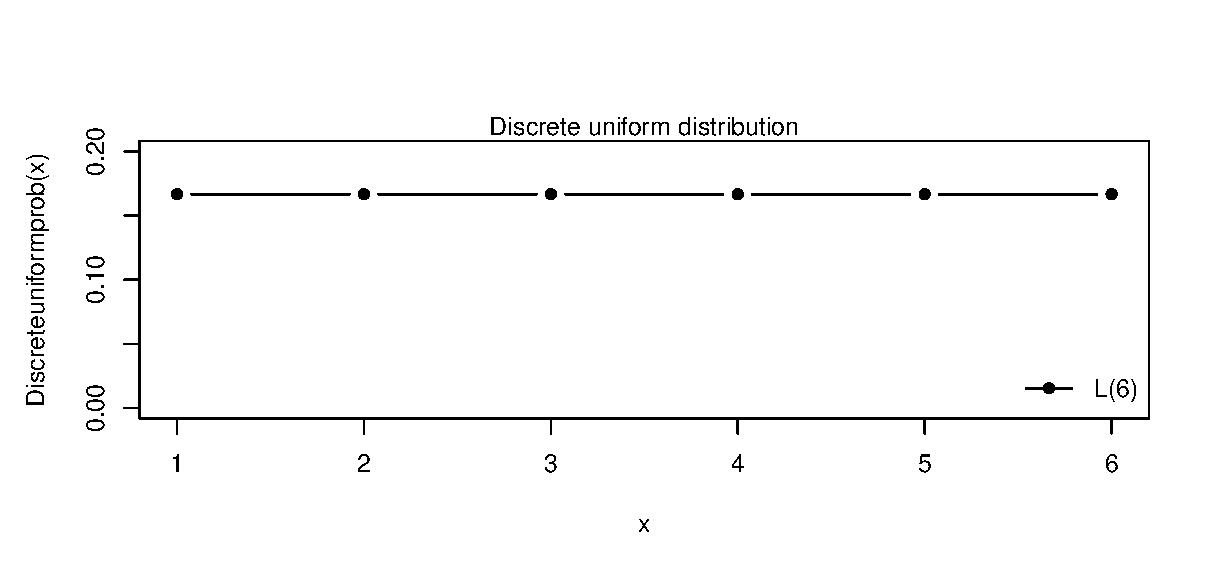
\includegraphics[scale=0.8]{lprob.eps}
\end{center}
\caption{Probability function of the discrete uniform distribution 
according to Eq.~(\ref{eq:lprob}) for the case $L(6)$. An
enveloping line is also shown.}
\lb{fig:lprob}
\end{figure}
%

\medskip
\noindent
Cumulative distribution function (\texttt{cdf}):
%
\be
\fbox{$\displaystyle
F_{X}(x) = P(X \leq x) = \sum_{i|x_{i}\leq x}\frac{1}{n} \ .
$}
\ee
%
Expectation value and variance:
%
\bea
\mathrm{E}(X) & = & \sum_{i=1}^{n}x_{i} \times \frac{1}{n}
= \mu \\
\mathrm{Var}(X) & = & \left(\sum_{i=1}^{n}x_{i}^{2} \times
\frac{1}{n}\right) - \mu^{2} \ .
\eea
%
For skewness and excess kurtosis, see, e.g., Rinne
(2008)~\ct[p~372f]{rin2008}.

\medskip
\noindent
The discrete uniform distribution is identical to a Laplacian 
probability measure; cf. Sec.~\ref{sec:laplace}. This is 
well-known from games of chance such as tossing a fair coin once, 
selecting a single card from a deck of cards, rolling a fair dye 
once, or the fair roulette lottery.

\medskip
\noindent
\underline{\R:} $\texttt{ddunif}(x,x_{1},x_{n})$,
$\texttt{pdunif}(x,x_{1},x_{n})$, 
$\texttt{qdunif}(\alpha,x_{1},x_{n})$,
$\texttt{rdunif}(n_{\mathrm{simulations}},x_{1},x_{n})$ (package:
{\tt extraDistr}, by Wolodzko (2018)~\ct{wol2018})

%%%%%%%%%%%%%%%%%%%%%%%%%%%%%%%%%%%%%%%%%%%%%%%%%%%%%%%%%%%%%%%%%%%
\section[Binomial distribution]{Binomial distribution}
\lb{sec:binomverteil}
%%%%%%%%%%%%%%%%%%%%%%%%%%%%%%%%%%%%%%%%%%%%%%%%%%%%%%%%%%%%%%%%%%%
%------------------------------------------------------------------
\subsection[Bernoulli distribution]{Bernoulli distribution}
%------------------------------------------------------------------
Another simple probability distribution, for a discrete 
one-dimensional random variable $X$ with only two possible values, 
$0$ and $1$,\footnote{Any one-dimensional random variable of this 
kind is referred to as dichotomous.} is due to the Swiss 
mathematician 
\href{http://www-history.mcs.st-and.ac.uk/Biographies/Bernoulli_Jacob.html}{Jakob Bernoulli (1654--1705)}. The \textbf{Bernoulli 
distribution},
%
\be
X \sim B(1;p) \ ,
\ee
%
depends on a single free parameter, the probability $p \in [0;1]$
for the event $X=1$.

\medskip
\noindent
Spectrum of values:
%
\be
X \mapsto x \in \left\{0, 1\right\} \ .
\ee
%
Probability function:
%
\be
\lb{eq:bprob}
\fbox{$\displaystyle
P(X=x) = \left(\begin{array}{c}
               1 \\
               x
               \end{array}\right)p^{x}(1-p)^{1-x} \ ,
\quad\text{with}\quad 0 \leq p \leq 1 \ ;
$}
\ee
%
its graph is shown in Fig.~\ref{fig:bprob} below for 
$\displaystyle p=\frac{1}{3}$.
%
\begin{figure}[!htb]
\begin{center}
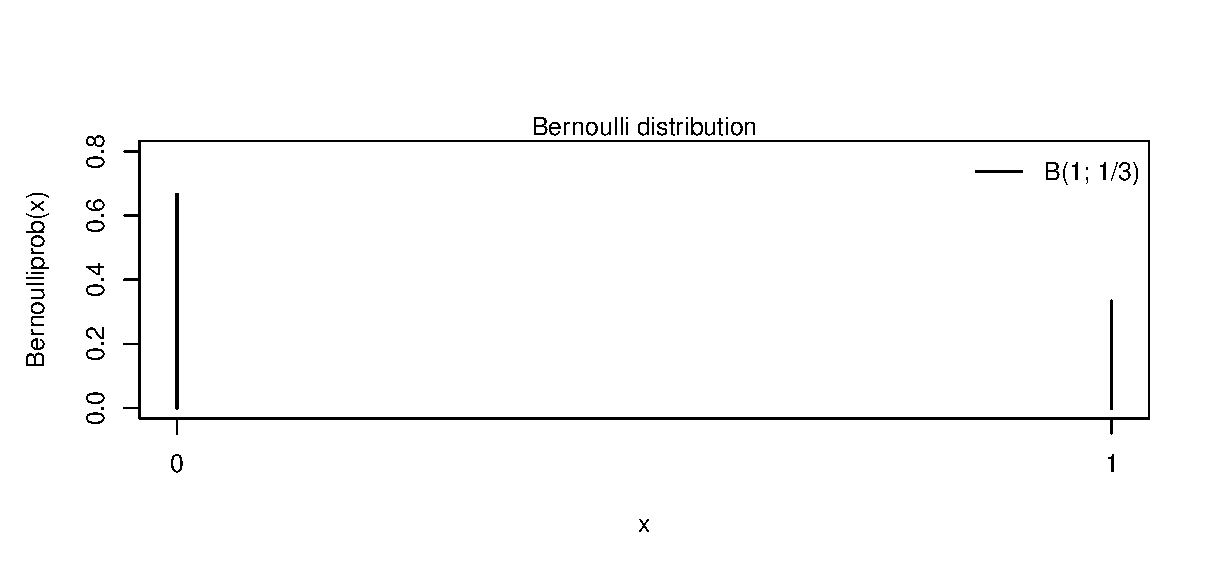
\includegraphics[scale=0.8]{bprob.eps}
\end{center}
\caption{Probability function of the Bernoulli distribution 
according to Eq.~(\ref{eq:bprob}) for the case $\displaystyle 
B\left(1;\frac{1}{3}\right)$.}
\lb{fig:bprob}
\end{figure}
%

\medskip
\noindent
Cumulative distribution function (\texttt{cdf}):
%
\be
\fbox{$\displaystyle
F_{X}(x) = P(X \leq x)
= \sum_{k=0}^{\left\lfloor x\right\rfloor}
\left(\begin{array}{c}
1 \\
k
\end{array}\right)p^{k}(1-p)^{1-k} \ .
$}
\ee
%
Expectation value and variance:
%
\bea
\mathrm{E}(X) & = & 0\times(1-p)+1\times p \ = \ p \\
\mathrm{Var}(X) & = & 0^{2}\times(1-p)+1^{2}\times p - p^{2}
\ = \ p(1-p) \ .
\eea
%

%------------------------------------------------------------------
\subsection[General binomial distribution]{General binomial
distribution}
%------------------------------------------------------------------
A direct generalisation of the Bernoulli distribution is the 
case of a discrete one-dimensional random variable $X$ which is 
the \textit{sum} of $n$ mutually stochastically independent, 
identically Bernoulli-distributed (``i.i.d.'') one-dimensional 
random variables $X_{i}\sim B(1;p)$ ($i=1,\ldots,n$), i.e.,
%
\be
X:=\sum_{i=1}^{n}X_{i}=X_{1}+\ldots +X_{n} \ ,
\ee
%
which yields the reproductive two-parameter \textbf{binomial 
distribution}
%
\be
X \sim B(n;p) \ ,
\ee
%
again with $p \in [0;1]$ the probability for a single event 
$X_{i}=1$.

\medskip
\noindent
Spectrum of values:
%
\be
X \mapsto x \in \left\{0, \ldots, n\right\} \ , 
\quad\quad\text{with}\quad n \in \mathbb{N} \ .
\ee
%
Probability function:\footnote{In the context of an urn model with 
$M$ black balls and $N-M$ white balls, and the random selection of 
$n$ balls from a total of $N$, with repetition, this probability 
function can be derived from Laplace's principle of forming the 
ratio between the ``number of favourable cases'' and the ``number 
of all possible cases,'' cf. Eq.~(\ref{eq:classprob}). Thus,
$\displaystyle P(X=x) = \frac{\left(\begin{array}{c}
n \\
x
\end{array}\right)M^{x}(N-M)^{n-x}}{N^{n}}$,
where $x$ denotes the number of black balls drawn, and one 
substitutes accordingly from the definition $p:=M/N$.}
%
\be
\lb{eq:binomialprob}
\fbox{$\displaystyle
P(X=x) = \left(\begin{array}{c}
               n \\
               x
               \end{array}\right)p^{x}(1-p)^{n-x} \ ,
\quad\quad\text{with}\quad 0 \leq p \leq 1 \ ;
$}
\ee
%
its graph is shown in Fig.~\ref{fig:biprob} below for 
$n=10$ and $\displaystyle p=\frac{3}{5}$. Recall that 
$\left(\begin{array}{c} n \\ x \end{array}\right)$ denotes the 
binomial coefficient defined in Eq.~(\ref{eq:binomcoeff}), which
generates the positive integer entries of Pascal's triangle.
%
\begin{figure}[!htb]
\begin{center}
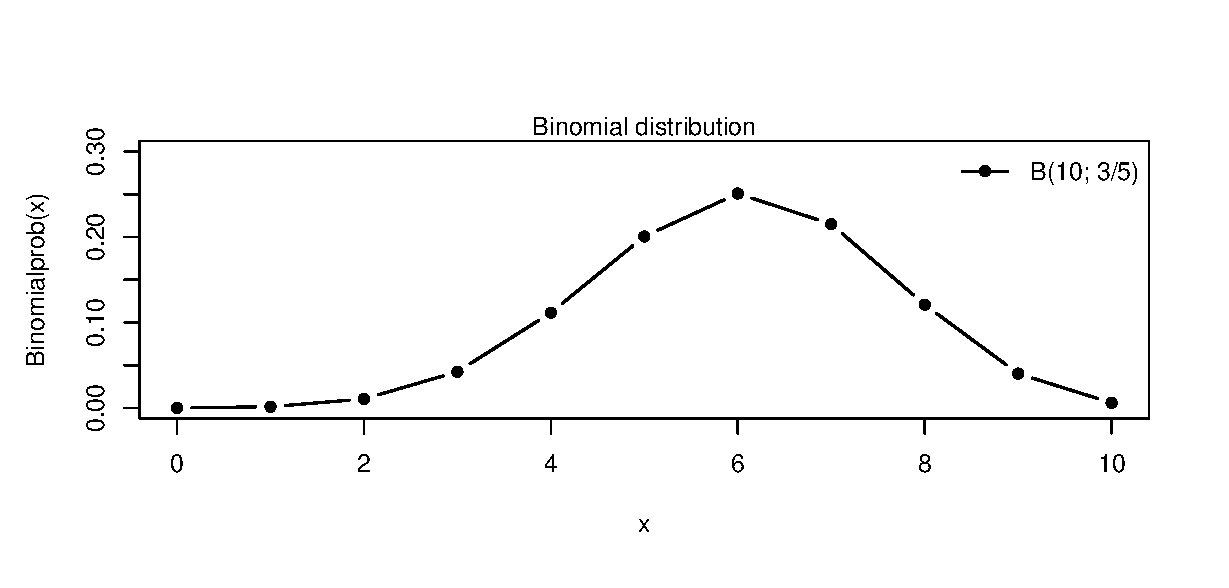
\includegraphics[scale=0.8]{biprob.eps}
\end{center}
\caption{Probability function of the binomial distribution 
according to Eq.~(\ref{eq:binomialprob}) for the case 
$\displaystyle B\left(10;\frac{3}{5}\right)$. An enveloping line is
also shown.}
\lb{fig:biprob}
\end{figure}
%

\medskip
\noindent
Cumulative distribution function (\texttt{cdf}):
%
\be
\fbox{$\displaystyle
F_{X}(x) = P(X \leq x)
= \sum_{k=0}^{\left\lfloor x\right\rfloor}
\left(\begin{array}{c}
n \\
k
\end{array}\right)p^{k}(1-p)^{n-k} \ .
$}
\ee
%
Expectation value, variance, skewness and excess kurtosis (cf. 
Rinne (2008)~\ct[p~260]{rin2008}):
%
\bea
\mathrm{E}(X) & = & \sum_{i=1}^{n}p \ = \ np \\
%
\mathrm{Var}(X) & = & \sum_{i=1}^{n}p(1-p) \ = \ np(1-p) \\
%
\mathrm{Skew}(X) & = & \frac{1-2p}{\sqrt{np(1-p)}} \\
%
\mathrm{Kurt}(X) & = & \frac{1-6p(1-p)}{np(1-p)} \ .
\eea
%
The results for $\mathrm{E}(X)$ and $\mathrm{Var}(X)$ are based on
the rules (\ref{eq:sumexpv}) and (\ref{eq:sumvar}), the latter of 
which applies to a set of mutually stochastically independent
random variables.

\medskip
\noindent
\underline{\R:} $\texttt{dbinom}(x,n,p)$, $\texttt{pbinom}(x,n,p)$, 
$\texttt{qbinom}(\alpha,n,p)$,
$\texttt{rbinom}(n_{\mathrm{simulations}},n,p)$ \\
\underline{GDC:} \texttt{binompdf}$(n,p,x)$,
\texttt{binomcdf}$(n,p,x)$ \\
\underline{EXCEL, OpenOffice:} \texttt{BINOM.DIST} (dt.:
\texttt{BINOM.VERT}, \texttt{BINOMVERT}), \texttt{BINOM.INV} (for 
$\alpha$--quantiles)

%%%%%%%%%%%%%%%%%%%%%%%%%%%%%%%%%%%%%%%%%%%%%%%%%%%%%%%%%%%%%%%%%%%
\section[Hypergeometric distribution]{Hypergeometric distribution}
\lb{sec:hypgeomverteil}
%%%%%%%%%%%%%%%%%%%%%%%%%%%%%%%%%%%%%%%%%%%%%%%%%%%%%%%%%%%%%%%%%%%
The \textbf{hypergeometric distribution} for a discrete 
one-dimensional random variable $X$ derives from an urn model with 
$M$ black balls and $N-M$ white balls, and the random selection of 
$n$ balls from a total of $N$ ($n \leq N$), without repetition. If 
$X$ represents the number of black balls amongst the $n$ selected 
balls, it is subject to the three-parameter probability 
distribution
%
\be
X \sim H(n,M,N) \ .
\ee
%
In particular, this model forms the mathematical basis of the 
internationally popular National Lotteries ``6 out of 49,'' in 
which case there are $M=6$ winning numbers amongst a total of 
$N=49$ numbers, and $X \in \left\{0, 1, \ldots, 6\right\}$ counts 
the total of correctly guessed winning numbers on an individual 
gambler's lottery ticket.

\medskip
\noindent
Spectrum of values:
%
\be
X \mapsto x \in \left\{\max(0,n-(N-M)), \ldots,
\min(n,M)\right\} \ .
\ee
%
Probability function:
%
\be
\lb{eq:hypergeomprob}
\fbox{$\displaystyle
P(X=x) = \frac{\left(\begin{array}{c}
               M \\
               x
               \end{array}\right)
         \left(\begin{array}{c}
               N-M \\
               n-x
               \end{array}\right)}{
               \left(\begin{array}{c}
               N \\
               n
               \end{array}\right)} \ ;
$}
\ee
%
its graph is shown in Fig.~\ref{fig:hypergeomprob} below for 
the National Lotteries example, so $n=6$, $M=6$ and $N=49$.
%
\begin{figure}[!htb]
\begin{center}
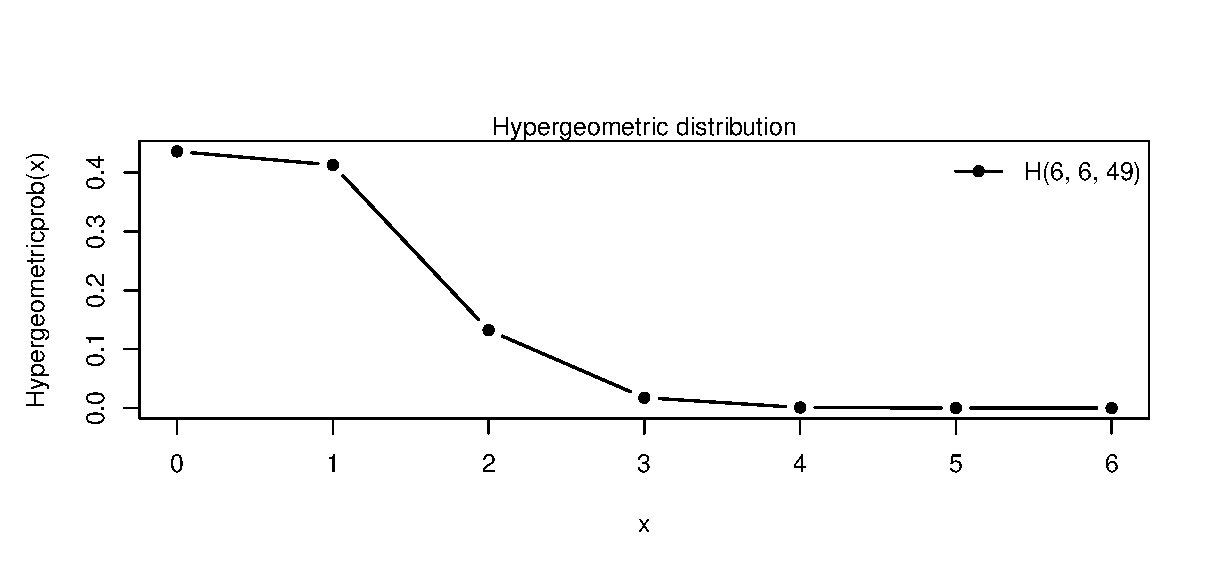
\includegraphics[scale=0.8]{hypergeomprob.eps}
\end{center}
\caption{Probability function of the hypergeometric distribution 
according to Eq.~(\ref{eq:hypergeomprob}) for the case 
$H\left(6,6,49\right)$. An enveloping line is also shown.}
\lb{fig:hypergeomprob}
\end{figure}
%

\medskip
\noindent
Cumulative distribution function (\texttt{cdf}):
%
\be
\fbox{$\displaystyle
F_{X}(x) = P(X \leq x)
= \sum_{k=\max(0,n-(N-M))}^{\left\lfloor x\right\rfloor}
\frac{\left(\begin{array}{c}
               M \\
               k
               \end{array}\right)
         \left(\begin{array}{c}
               N-M \\
               n-k
               \end{array}\right)}{
               \left(\begin{array}{c}
               N \\
               n
               \end{array}\right)} \ .
$}
\ee
%
Expectation value and variance:
%
\bea
\mathrm{E}(X) & = & n\,\frac{M}{N} \\
\mathrm{Var}(X) & = & n\,\frac{M}{N}\left(1-\frac{M}{N}\right)
\left(\frac{N-n}{N-1}\right) \ .
\eea
%
For skewness and excess kurtosis, see, e.g., Rinne
(2008)~\ct[p~270]{rin2008}.

\medskip
\noindent
\underline{\R:} $\texttt{dhyper}(x,M,N-M,n)$,
$\texttt{phyper}(x,M,N-M,n)$,
$\texttt{qhyper}(\alpha,M,N-M,n)$, \\
$\texttt{rhyper}(n_{\mathrm{simulations}},M,N-M,n)$ \\
\underline{EXCEL, OpenOffice:} \texttt{HYPGEOM.DIST}
(dt.: \texttt{HYPGEOM.VERT}, \texttt{HYPGEOMVERT})

%%%%%%%%%%%%%%%%%%%%%%%%%%%%%%%%%%%%%%%%%%%%%%%%%%%%%%%%%%%%%%%%%%%
\section[Poisson distribution]{Poisson distribution}
\lb{sec:poissonverteil}
%%%%%%%%%%%%%%%%%%%%%%%%%%%%%%%%%%%%%%%%%%%%%%%%%%%%%%%%%%%%%%%%%%%
The one-parameter \textbf{Poisson distribution} for a discrete 
one-dimensional random variable $X$,
%
\be
X \sim Pois(\lambda) \ .
\ee
%
plays a major role in analysing \textbf{count data} when the
maximum number of possible counts associated with a corresponding
data-generating process is unknown. This distribution is named
after the French mathematician, engineer, and physicist 
\href{http://www-history.mcs.st-and.ac.uk/Biographies/Poisson.html}{Baron
Sim\'{e}on Denis Poisson FRSFor HFRSE MIF (1781--1840)} and can be
considered a special case of the binomial distribution, discussed
in Sec.~\ref{sec:binomverteil}, when $n$ is very large ($n \gg 1$)
and $p$ is very small ($0 < p \ll 1$); cf. Sivia and Skilling
(2006)~\ct[Sec.~5.4]{sivski2006}.

\medskip
\noindent
Spectrum of values:
%
\be
X \mapsto x \in \left\{0, \ldots, n\right\} \ , 
\quad\quad\text{with}\quad n \in \mathbb{N} \ . \ .
\ee
%
Probability function:
%
\be
\lb{eq:poissonprob}
\fbox{$\displaystyle
P(X=x) = \frac{\lambda^{x}}{x!}\exp\left(-\lambda\right) \ ,
\quad\text{with}\quad \lambda \in \mathbb{R}_{>0}\ ;
$}
\ee
%
$\lambda$ is a dimensionless rate parameter. It is also  referred
to as the intensity parameter. The graph of the probability
function is shown in Fig.~\ref{fig:poissonprob} below for the case
$\displaystyle\lambda=\frac{3}{2}$.
%
\begin{figure}[!htb]
\begin{center}
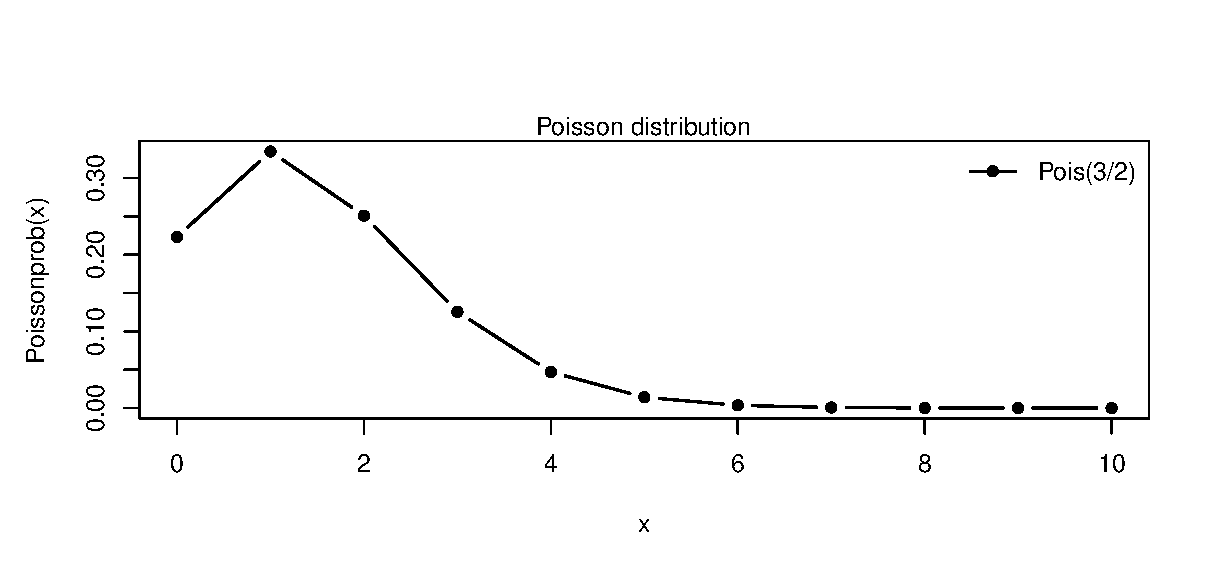
\includegraphics[scale=0.8]{poissonprob.eps}
\end{center}
\caption{Probability function of the Poisson distribution 
according to Eq.~(\ref{eq:poissonprob}) for the case 
$\displaystyle Pois\left(\frac{3}{2}\right)$. An enveloping line is
also shown.}
\lb{fig:poissonprob}
\end{figure}
%

\medskip
\noindent
Cumulative distribution function (\texttt{cdf}):
%
\be
\fbox{$\displaystyle
F_{X}(x) = P(X \leq x)
= \left(\sum_{k=0}^{\left\lfloor x\right\rfloor}
\frac{\lambda^{k}}{k!}\right)\exp\left(-\lambda\right) \ .
$}
\ee
%
Expectation value, variance, skewness and excess kurtosis (cf. 
Rinne (2008)~\ct[p~285f]{rin2008}):\footnote{Note that for a
binomial distribution, cf. Sec.~\ref{sec:binomverteil}, in the
limit that $n \gg 1$ while simultaneously $0 < p \ll 1$ it holds
that $np \approx np(1-p)$, and so the corresponding expectation
value and variance become more and more equal.}
%
\bea
\mathrm{E}(X) & = & \lambda \\
%
\mathrm{Var}(X) & = & \lambda \\
%
\mathrm{Skew}(X) & = & \frac{1}{\sqrt{\lambda}} \\
%
\mathrm{Kurt}(X) & = & \frac{1}{\lambda} \ .
\eea
%

\medskip
\noindent
\underline{\R:} $\texttt{dpois}(x,\lambda)$,
$\texttt{ppois}(x,\lambda)$, $\texttt{qpois}(\alpha,\lambda)$,
$\texttt{rpois}(n_{\mathrm{simulations}},\lambda)$ \\
\underline{EXCEL, OpenOffice:} \texttt{POISSON.DIST}
(dt.: \texttt{POISSON.VERT}), \texttt{POISSON}

%%%%%%%%%%%%%%%%%%%%%%%%%%%%%%%%%%%%%%%%%%%%%%%%%%%%%%%%%%%%%%%%%%%
\section[Continuous uniform distribution]{Continuous uniform
distribution}
\lb{sec:sgleichverteil}
%%%%%%%%%%%%%%%%%%%%%%%%%%%%%%%%%%%%%%%%%%%%%%%%%%%%%%%%%%%%%%%%%%%
The simplest example of a probability distribution for a 
continuous one-dimensional random variable $X$ is the
\textbf{continuous uniform distribution},
%
\be
X \sim U(a;b) \ ,
\ee
%
also referred to as the \textbf{rectangular distribution}. Its two 
free parameters, $a$ and $b$, denote the limits of $X$'s

\medskip
\noindent
Spectrum of values:
%
\be
X \mapsto x \in \left[a,b\right]
\subset \mathbb{R} \ .
\ee
%
Probability density function (\texttt{pdf}):\footnote{It is a nice 
and instructive little exercise, strongly recommended to the 
reader, to go through the details of explicitly computing from 
this simple \texttt{pdf} the corresponding \texttt{cdf}, expectation 
value, variance, skewness and excess kurtosis of $X \sim U(a;b)$.}
%
\be
\lb{eq:recpdf}
\fbox{$\displaystyle
f_{X}(x) =
\begin{cases}
{\displaystyle \frac{1}{b-a}} &
\text{for}\quad x \in \left[a,b\right] \\
\\
0 & \text{otherwise}
\end{cases} \ ;
$}
\ee
%
its graph is shown in Fig.~\ref{fig:unifpdf} below for three 
different combinations of the parameters $a$ and $b$.
%
\begin{figure}[!htb]
\begin{center}
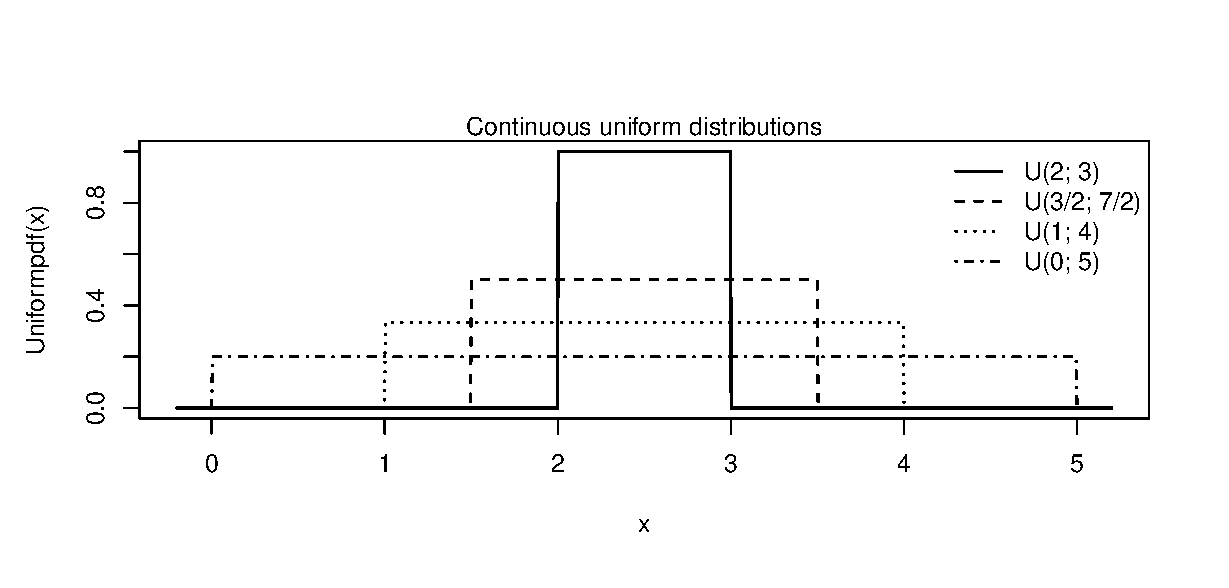
\includegraphics[scale=0.8]{unifpdf.eps}
\end{center}
\caption{\texttt{pdf} of the continuous uniform distribution 
according to Eq.~(\ref{eq:recpdf}) for the cases $U(0;5)$, 
$U(1;4)$, $U(3/2;7/2)$ and $U(2;3)$.}
\lb{fig:unifpdf}
\end{figure}
%

\medskip
\noindent
Cumulative distribution function (\texttt{cdf}):
%
\be
\lb{eq:reccdf}
\fbox{$\displaystyle
F_{X}(x) = P(X \leq x) =
\begin{cases}
0 & \text{for}\quad x < a \\ \\
{\displaystyle \frac{x-a}{b-a}} &
\text{for}\quad x \in \left[a,b\right] \\ \\
1 & \text{for}\quad x > b
\end{cases} \ .
$}
\ee
%
Expectation value, variance, skewness and excess kurtosis:
%
\bea
% Skewness and excess kurtosis results explicitly verified on
% Mi, 14.08.2013.
\mathrm{E}(X) & = & \frac{a+b}{2} \\
%
\lb{eq:varUniDistr}
\mathrm{Var}(X) & = & \frac{(b-a)^{2}}{12} \\
%
\mathrm{Skew}(X) & = & 0 \\
%
\mathrm{Kurt}(X) & = & -\,\frac{6}{5} \ .
\eea
%
Using some of these results, as well as Eq.~(\ref{eq:reccdf}), one 
finds that for all continuous uniform distributions the event 
probability
%
\bea
P(|X-\mathrm{E}(X)| \leq \sqrt{\mathrm{Var}(X)})
& = & P\left(\frac{\sqrt{3}(a+b)-(b-a)}{2\sqrt{3}}
\leq X \leq
\frac{\sqrt{3}(a+b)+(b-a)}{2\sqrt{3}}\right) \nonumber \\
& = & \frac{1}{\sqrt{3}} \ \approx\ 0.5773 \ ,
\eea
%
i.e., the event probability that $X$ falls within one standard 
deviation (``$1\sigma$'') of $\mathrm{E}(X)$ is $1/\sqrt{3}$. 
$\alpha$--quantiles of continuous uniform distributions are 
obtained by straightforward inversion, i.e., for $0 < \alpha < 1$,
%
\be
\alpha \stackrel{!}{=} F_{X}(x_{\alpha})
= \frac{x_{\alpha}-a}{b-a}
\qquad\Leftrightarrow\qquad
x_{\alpha} = F_{X}^{-1}(\alpha) = a + \alpha(b-a) \ .
\ee
%

\medskip
\noindent
\underline{\R:} $\texttt{dunif}(x,a,b)$,
$\texttt{punif}(x,a,b)$, $\texttt{qunif}(\alpha,a,b)$,
$\texttt{runif}(n_{\mathrm{simulations}},a,b)$

\medskip
\noindent
Standardisation of $X \sim U(a;b)$ according to
Eq.~(\ref{eq:standardisation}) yields a one-dimensional random 
variable $Z \sim U(-\sqrt{3};\sqrt{3})$ by
%
\be
X \rightarrow Z = \sqrt{3}\,\frac{2X-(a+b)}{b-a}
\mapsto z \in \left[-\sqrt{3}, \sqrt{3}\right] \ ,
\ee
%
with $\texttt{pdf}$
%
\be
f_{Z}(z) =
\begin{cases}
{\displaystyle \frac{1}{2\sqrt{3}}} & \text{for}\quad z \in
\left[-\sqrt{3}, \sqrt{3}\right] \\ \\
0 & \text{otherwise}
\end{cases} \ ,
\ee
%
and $\texttt{cdf}$
%
\be
F_{Z}(z) = P(Z \leq z) =
\begin{cases}
0 & \text{for}\quad z < -\sqrt{3} \\ \\
{\displaystyle \frac{z+\sqrt{3}}{2\sqrt{3}}} &
\text{for}\quad z \in \left[-\sqrt{3},\sqrt{3}\right] \\ \\
1 & \text{for}\quad z > \sqrt{3}
\end{cases} \ .
\ee
%

%%%%%%%%%%%%%%%%%%%%%%%%%%%%%%%%%%%%%%%%%%%%%%%%%%%%%%%%%%%%%%%%%%%
\section[Gau\ss ian normal distribution]{\href{https://www.youtube.com/watch?v=8fjDkBT641o}{Gau\ss ian normal distribution}}
\lb{sec:normverteil}
%%%%%%%%%%%%%%%%%%%%%%%%%%%%%%%%%%%%%%%%%%%%%%%%%%%%%%%%%%%%%%%%%%%
The best-known probability distribution for a continuous
one-dimensional random variable $X$, 
which proves ubiquitous in \textbf{Inferential Statistics} (see
Chs. \ref{ch12}  and \ref{ch13} below), is due to 
\href{http://www-groups.dcs.st-and.ac.uk/~history/Biographies/Gauss.html}{Carl Friedrich Gau\ss\ (1777--1855)}; cf. Gau\ss\ 
(1809)~\ct{gau1809}. This is the reproductive two-parameter
\textbf{normal distribution}
%
\be
X \sim N(\mu;\sigma^{2}) \ ;
\ee
%
the meaning of the parameters $\mu$ and $\sigma^{2}$ will be 
explained shortly. The extraordinary status of the \textbf{normal 
distribution} in \textbf{Probability Theory} and
\textbf{Statistics} was cemented through the discovery of the
\textbf{central limit theorem} by the French mathematician and
astronomer
\href{http://www-history.mcs.st-and.ac.uk/Biographies/Laplace.html}{Marquis Pierre Simon de Laplace (1749--1827)}, cf. Laplace 
(1809)~\ct{lap1809}; see Sec.~\ref{sec:zentrgrenz} below.

\medskip
\noindent
Spectrum of values:
%
\be
X \mapsto x \in D \subseteq \mathbb{R} \ .
\ee
%
Probability density function (\texttt{pdf}):
%
\be
\lb{glockenpdf}
\fbox{$\displaystyle
f_{X}(x) = \frac{1}{\sqrt{2\pi}\sigma}\exp\left[-\frac{1}{2}
\left(\frac{x-\mu}{\sigma}\right)^{2}\right] \ ,
\quad\text{with}\quad \sigma \in \mathbb{R}_{>0} \ .
$}
\ee
%
This normal--\texttt{pdf} defines a reflection-symmetric 
characteristic bell-shaped curve, the analytical properties of 
which were first discussed by the French mathematician 
\href{http://www-history.mcs.st-and.ac.uk/Biographies/De_Moivre.html}{Abraham de Moivre (1667--1754)}. The $x$--position of this 
curve's (global) maximum is specified by $\mu$, while the 
$x$--positions of its two points of inflection are given by 
$\mu-\sigma$ resp.~$\mu+\sigma$. The effects of different values 
of the parameters $\mu$ and $\sigma$ on the bell-shaped curve are 
illustrated in Figs.~\ref{fig:norm1pdf} and~\ref{fig:norm2pdf}
below.
%
\begin{figure}[!htb]
\begin{center}
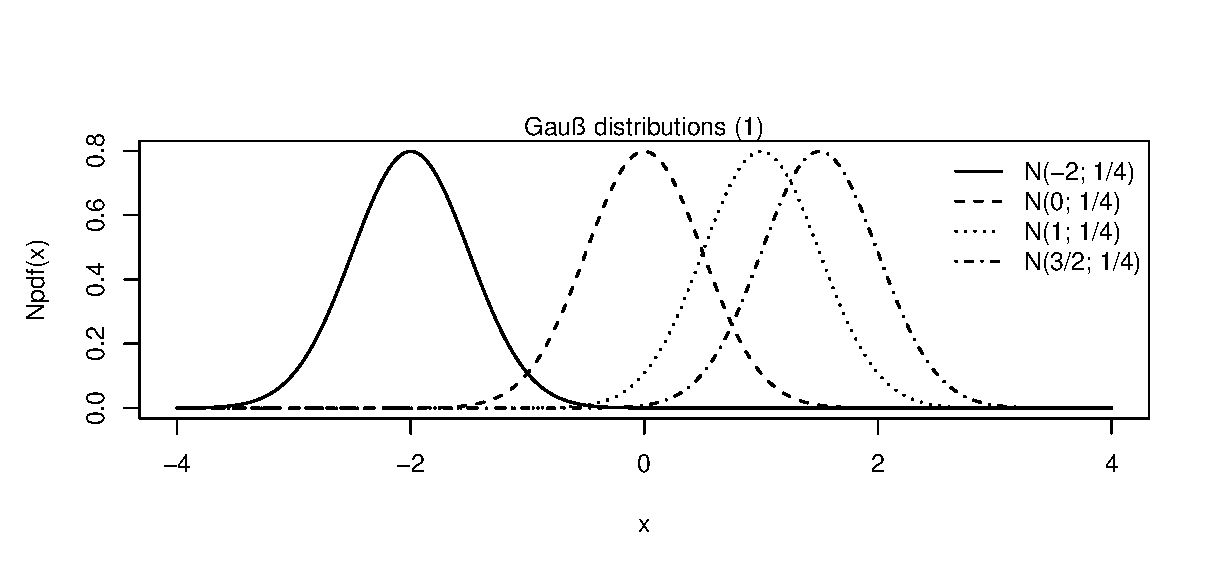
\includegraphics[scale=0.8]{norm1pdf.eps}
\end{center}
\caption{\texttt{pdf} of the Gau\ss ian normal distribution
according to Eq.~(\ref{glockenpdf}). Cases $N(-2;1/4)$,
$N(0;1/4)$, $N(1;1/4)$ and $N(3/2;1/4)$, which have
constant~$\sigma$.}
\lb{fig:norm1pdf}
\end{figure}
%
%
\begin{figure}[!htb]
\begin{center}
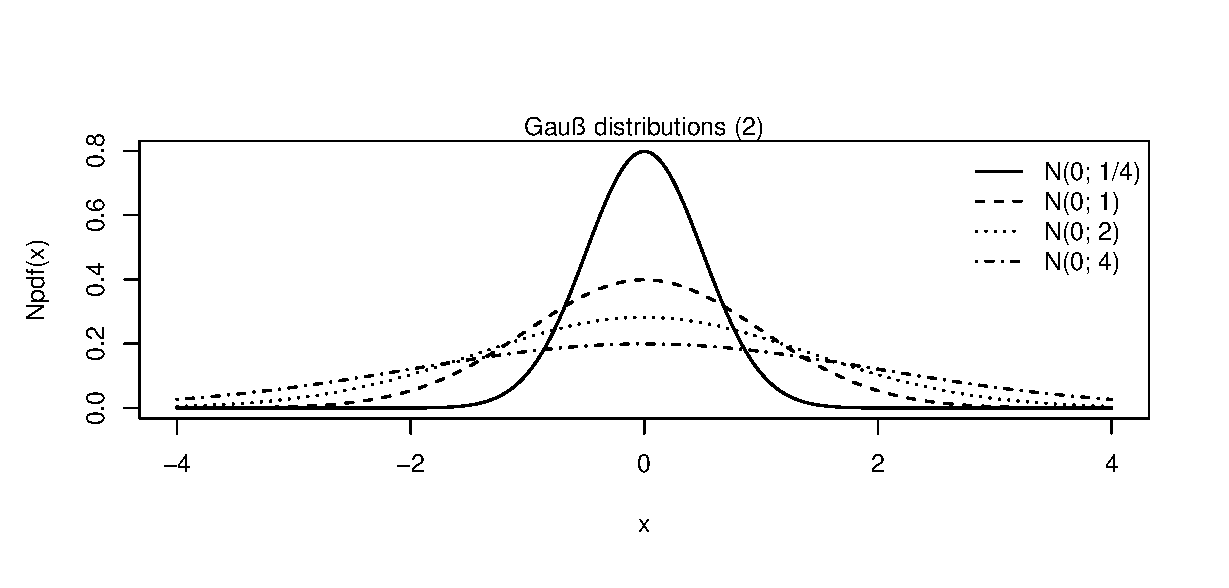
\includegraphics[scale=0.8]{norm2pdf.eps}
\end{center}
\caption{\texttt{pdf} of the Gau\ss ian normal distribution
according to Eq.~(\ref{glockenpdf}). Cases $N(0;1/4)$, $N(0;1)$,
$N(0;2)$ and $N(0;4)$, which have constant~$\mu$.}
\lb{fig:norm2pdf}
\end{figure}
%

\medskip
\noindent
Cumulative distribution function (\texttt{cdf}):
%
\be
\lb{eq:gaussiancdf}
\fbox{$\displaystyle
F_{X}(x) = P (X \leq x) = \int_{-\infty}^{x}
\frac{1}{\sqrt{2\pi}\sigma}\exp\left[-\frac{1}{2}
\left(\frac{t-\mu}{\sigma}\right)^{2}\right]\mathrm{d}t \ .
$}
\ee
%
We emphasise the fact that the normal--\texttt{cdf} \textit{cannot}
be expressed in terms of elementary mathematical functions.

\medskip
\noindent
Expectation value, variance, skewness and excess kurtosis (cf. 
Rinne (2008)~\ct[p~301]{rin2008}):
%
\bea
\mathrm{E}(X) & = & \mu \\
%
\mathrm{Var}(X) & = & \sigma^{2} \\
%
\mathrm{Skew}(X) & = & 0 \\
%
\mathrm{Kurt}(X) & = & 0 \ .
\eea
%

\medskip
\noindent
\underline{\R:} $\texttt{dnorm}(x,\mu,\sigma)$,
$\texttt{pnorm}(x,\mu,\sigma)$,
$\texttt{qnorm}(\alpha,\mu,\sigma)$,
$\texttt{rnorm}(n_{\mathrm{simulations}},\mu,\sigma)$ \\
\underline{GDC:} \texttt{normalpdf}$(x,\mu,\sigma)$,
\texttt{normalcdf}$(-\infty,x,\mu,\sigma)$ \\
\underline{EXCEL, OpenOffice:} \texttt{NORM.DIST} (dt.:
\texttt{NORM.VERT}, \texttt{NORMVERT})

\vspace{5mm}
\noindent
Upon standardisation of a normally distributed one-dimensional 
random variable $X$ according to Eq.~(\ref{eq:standardisation}), 
the cor\-responding normal distribution $N(\mu;\sigma^{2})$ is 
transformed into the unique \textbf{standard normal distribution}, 
$N(0;1)$, with

\medskip
\noindent
Probability density function (\texttt{pdf}):
%
\be
\lb{sglockenpdf}
\fbox{$\displaystyle
\varphi(z) := \frac{1}{\sqrt{2\pi}}\exp\left[-\frac{1}{2}\,z^{2}
\right] \quad\text{for}\quad
z \in \mathbb{R} \ ;
$}
\ee
%
its graph is shown in Fig.~\ref{fig:snormpdf} below.
%
\begin{figure}[!htb]
\begin{center}
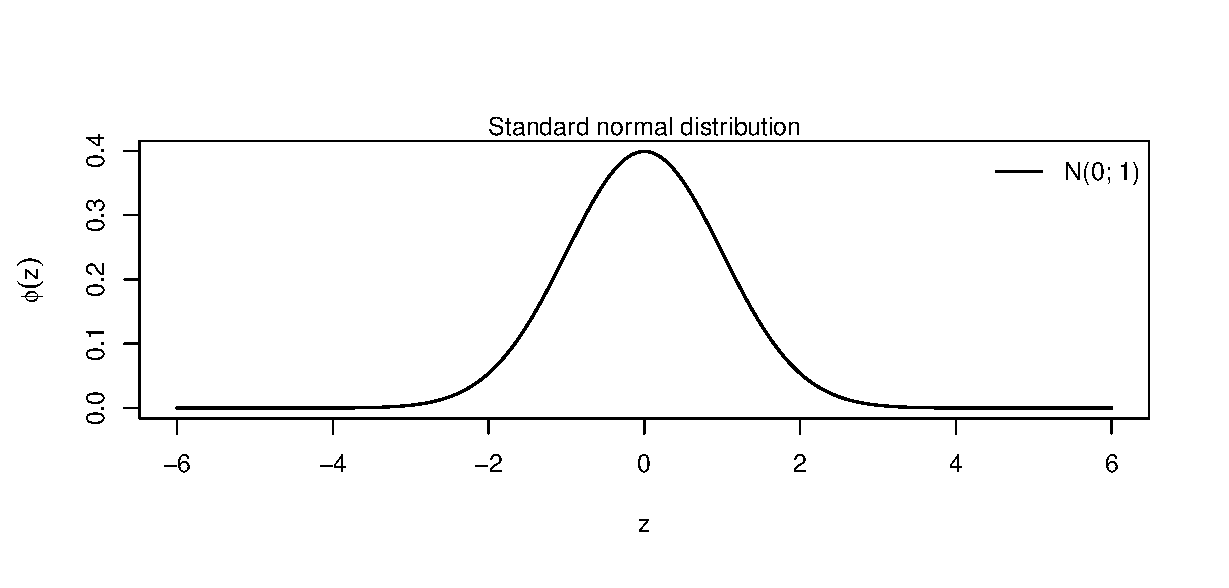
\includegraphics[scale=0.8]{snormpdf.eps}
\end{center}
\caption{\texttt{pdf} of the standard normal distribution according 
to Eq.~(\ref{sglockenpdf}).}
\lb{fig:snormpdf}
\end{figure}
%

\medskip
\noindent
Cumulative distribution function (\texttt{cdf}):
%
\be
\fbox{$\displaystyle
\Phi(z) := P(Z \leq z) = \int_{-\infty}^{z}
\frac{1}{\sqrt{2\pi}}\exp\left[-\frac{1}{2}\,t^{2}\right]
\mathrm{d}t \ .
$}
\ee
%

\medskip
\noindent
\underline{\R:} $\texttt{dnorm}(z)$,
$\texttt{pnorm}(z)$, $\texttt{qnorm}(\alpha)$,
$\texttt{rnorm}(n_{\mathrm{simulations}})$ \\
\underline{EXCEL:} \texttt{NORM.S.DIST} (dt.: \texttt{NORM.S.VERT})

\vspace{5mm}
\noindent
The resultant random variable $Z \sim N(0;1)$ satisfies the

\medskip
\noindent
Computational rules:
%
\bea
P(Z \leq b) & = & \Phi(b) \\
%
P(Z \geq a) & = & 1-\Phi(a) \\
%
P(a \leq Z \leq b) & = & \Phi(b) - \Phi(a) \\
%
\Phi(-z) & = & 1 - \Phi(z) \\
%
\lb{eq:symzint}
P(-z \leq Z \leq z) & = & 2\Phi(z) - 1 \ .
\eea
%
The event probability that a (standard) normally distributed 
one-dimensional random variable %$Z \sim N(0;1)$
takes values inside an interval of length $k$ times two standard 
deviations, %(where $\sqrt{\mathrm{Var}(Z)}=1$)
centred on its expectation value, is given by the important
$\boldsymbol{k}\boldsymbol{\sigma}$\textbf{--rule}. This states
that 
%
\be
P(|X-\mu| \leq k\sigma) 
\overbrace{=}^{{\text{Eq.~(\ref{eq:standardisation})}}}
P(-k \leq Z \leq +k)
\overbrace{=}^{{\text{Eq.~(\ref{eq:symzint})}}}
2\Phi(k) - 1 \quad \text{for}\quad k>0 \ .
\ee
%
According to this rule, the event probability of a normally 
distributed one-dimensional random variable to deviate from its 
mean by \textit{more than six standard deviations} amounts to
%
\be
P(|X-\mu| > 6\sigma) = 2\left[1-\Phi(6)\right]
\approx 1.97 \times 10^{-9} \ ,
\ee
%
i.e., about two parts in one billion. Thus, in this scenario 
the occurrence of extreme \textbf{outliers} for~$X$ is practically 
impossible. In turn, the persistent occurrence of so-called 
$\boldsymbol{6\sigma}$\textbf{--events}, or larger deviations from
the mean, in quantitative statistical surveys can be interpreted as
evidence \textit{against} the assumption of an underlying
Gau\ss ian random process; cf. Taleb (2007)~\ct[Ch.~15]{tal2007}.

\medskip
\noindent
The rapid, accelerated decline in the event probabilities for 
deviations from the mean of a  Gau\ss ian normal distribution can 
be related to the fact that the elasticity of the 
standard normal--\texttt{pdf} is given by (cf. 
Ref.~\ct[Sec.~7.6]{hve2009})
%
\be
\lb{eq:phielasts}
\varepsilon_{\varphi}(z) = -\,z^{2} \ .
%\quad\quad\text{resp.}\quad\quad
%\varepsilon_{\varphi}\left[\varepsilon_{\varphi}(z)\right] = 2 \ .
\ee
%
Manifestly this is negative for all $z \neq 0$ and increases
non-linearly in absolute value as one moves away from $z=0$.

\medskip
\noindent
$\alpha$--quantiles associated with $Z \sim N(0;1)$ are obtained
from the inverse standard normal--\texttt{cdf} according to
%
\be
\alpha \stackrel{!}{=} P(Z \leq z_{\alpha}) = \Phi(z_{\alpha})
\qquad\Leftrightarrow\qquad
z_{\alpha} = \Phi^{-1}(\alpha)
\quad\text{for\ all}\quad 0 < \alpha < 1 \ .
\ee
%
Due to the reflection symmetry of $\varphi(z)$ with respect to the
vertical axis at $z=0$, it holds that
%
\be
z_{\alpha} = -z_{1-\alpha} \ .
\ee
%
For this reason, one typically finds $z_{\alpha}$-values listed in 
textbooks on \textbf{Statistics} only for $\alpha \in [1/2,1)$. 
Alternatively, a particular $z_{\alpha}$ may be obtained from \R,
a GDC, EXCEL, or from OpenOffice. The backward transformation from
a particular $z_{\alpha}$ of the standard normal distribution to
the corresponding~$x_{\alpha}$ of a given normal distribution
follows from Eq.~(\ref{eq:standardisation}) and amounts to
$x_{\alpha} = \mu+z_{\alpha}\sigma$.

\medskip
\noindent
\underline{\R:} $\texttt{qnorm}(\alpha)$ \\
\underline{GDC:} \texttt{invNorm}$(\alpha)$ \\
\underline{EXCEL, OpenOffice:} \texttt{NORM.S.INV} (dt.:
\texttt{NORM.S.INV}, \texttt{NORMINV})

\vspace{5mm}
\noindent
At this stage, a few historical remarks are in order. The
Gau\ss ian normal distribution gained a prominent, though in 
parts questionable status in the \textbf{Social Sciences} through
the highly influential work of the Belgian astronomer, 
mathematician, statistician and sociologist 
\href{http://www-history.mcs.st-and.ac.uk/Biographies/Quetelet.html}{Lambert Adolphe Jacques Quetelet (1796--1874)} during the 
$19^\mathrm{th}$ Century. In particular, his research programme on 
the generic properties of \textit{l'homme moyen} (engl.: the
average man), see Quetelet (1835)~\ct{que1835}, an ambitious and to
some extent obsessive attempt to quantify and classify
physiological and sociological human characteristics according to
the principles of a normal distribution, left a lasting impact on
the field, with repercussions to this day. Quetelet, by the way,
co-founded the \href{http://www.rss.org.uk}{Royal Statistical
Society (\texttt{rss.org.uk})} in 1834. Further visibility was
given to Quetelet's ideas at the time by a contemporary, the
English empiricist 
\href{http://www-history.mcs.st-and.ac.uk/Biographies/Galton.html}{Sir Francis Galton FRS (1822--1911)}, whose intense studies on 
heredity in Humans, see Galton (1869)~\ct{gal1869}, which he later 
subsumed under the term ``eugenics,'' complemented Quetelet's 
investigations, and profoundly shaped subsequent developments in 
social research; cf. Bernstein (1998)~\ct[Ch.~9]{ber1998}. 
Incidently, amongst many other contributions to the field, 
Galton's activities helped to pave the way for making
\textbf{questionnaires} and \textbf{surveys} a commonplace for
collecting statistical data from Humans.

\vspace{5mm}
\noindent
The (standard) normal distribution, as well as the next three 
examples of probability distributions for a continuous
one-dimensional random variable $X$, are commonly referred to as
the \textbf{test distributions}, due to the central roles they play
in null hypothesis significance testing (cf. Chs. \ref{ch12} and
\ref{ch13}).

%%%%%%%%%%%%%%%%%%%%%%%%%%%%%%%%%%%%%%%%%%%%%%%%%%%%%%%%%%%%%%%%%%%
\section[$\chi^{2}$--distribution]{
$\boldsymbol{\chi}^{2}$--distribution with $n$ degrees of freedom}
\lb{sec:chi2verteil}
%%%%%%%%%%%%%%%%%%%%%%%%%%%%%%%%%%%%%%%%%%%%%%%%%%%%%%%%%%%%%%%%%%%
The reproductive one-parameter
$\boldsymbol{\chi}^{2}$\textbf{--distribution with}
$\boldsymbol{n}$ \textbf{degrees of freedom} was
devised by the English mathematical statistician 
\href{http://www-history.mcs.st-and.ac.uk/Biographies/Pearson.html}{Karl Pearson FRS (1857--1936)}; cf. Pearson (1900)~\ct{pea1900}. 
The underlying continuous one-dimensional random variable
%
\be
\fbox{$\displaystyle
X \sim \chi^{2}(n) \ ,
$}
\ee
%
is perceived of as the sum of squares of $n$ stochastically 
independent, identically standard normally distributed 
(``i.i.d.'') random variables $Z_{i} \sim N(0;1)$ 
($i=1,\ldots,n$), i.e.,
%
\be
X:=\sum_{i=1}^{n}Z_{i}^{2}
= Z_{1}^{2} + \ldots + Z_{n}^{2} \ ,
\quad\text{with}\quad n \in \mathbb{N} \ .
\ee
%

\medskip
\noindent
Spectrum of values:
%
\be
X \mapsto x \in D \subseteq \mathbb{R}_{\geq 0} \ .
\ee
%
The probability density function (\texttt{pdf}) of a 
$\chi^{2}$--distribution with $df=n$ degrees of freedom is a 
fairly complicated mathematical expression; see Rinne 
(2008)~\ct[p~319]{rin2008} or Ref.~\ct[Eq.~(3.26)]{hve2018} for the
explicit representation of the $\chi^{2}$\texttt{pdf}. Plots are
shown for four different values of the parameter $n$ in
Fig.~\ref{fig:chi2pdf}. The $\chi^{2}$\texttt{cdf} \textit{cannot}
be expressed in terms of elementary mathematical functions.
%
\begin{figure}[!htb]
\begin{center}
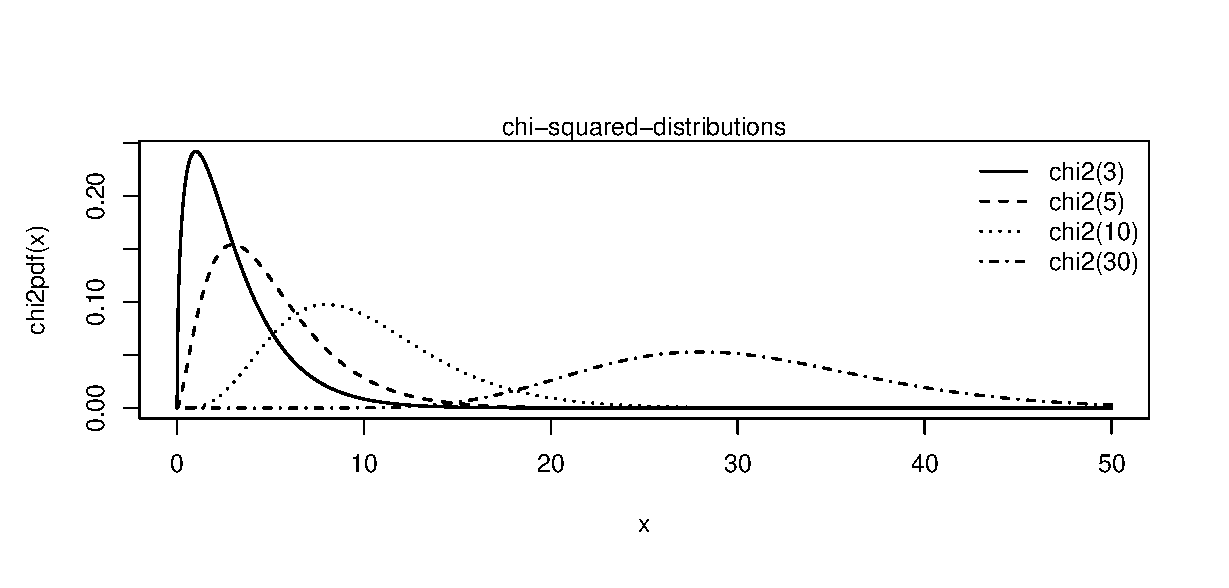
\includegraphics[scale=0.8]{chi2pdf.eps}
\end{center}
\caption{\texttt{pdf} of the $\chi^{2}$--distribution for $df=n \in 
\{3, 5, 10, 30\}$ degrees of freedom.}
\lb{fig:chi2pdf}
\end{figure}
%

\medskip
\noindent
Expectation value, variance, skewness and excess kurtosis (cf. 
Rinne (2008)~\ct[p~320f]{rin2008}):
%
\bea
\mathrm{E}(X) & = & n \\
%
\mathrm{Var}(X) & = & 2n \\
%
\mathrm{Skew}(X) & = & \sqrt{\frac{8}{n}} \\
%
\mathrm{Kurt}(X) & = & \frac{12}{n} \ .
\eea
%
$\alpha$--quantiles, $\chi^{2}_{n;\alpha}$, of 
$\chi^{2}$--distributions are generally tabulated in textbooks on 
\textbf{Statistics}. Alternatively, they may be obtained from \R,
EXCEL, or from OpenOffice.

\medskip
\noindent
Note that for $n \geq 50$ a $\chi^{2}(n)$--distribution may be 
approximated reasonably well by a normal distribution, $N(n,2n)$. 
This is a reflection of the \textbf{central limit theorem}, to be 
discussed in Sec.~\ref{sec:zentrgrenz} below.

\medskip
\noindent
\underline{\R:} $\texttt{dchisq}(x,n)$, $\texttt{pchisq}(x,n)$,
$\texttt{qchisq}(\alpha,n)$,
$\texttt{rchisq}(n_{\mathrm{simulations}},n)$ \\
\underline{GDC:} $\chi^{2}\texttt{pdf}(x,n)$,
$\chi^{2}\texttt{cdf}(0,x,n)$ \\
\underline{EXCEL, OpenOffice:} \texttt{CHISQ.DIST},
\texttt{CHISQ.INV} (dt.: \texttt{CHIQU.VERT}, \texttt{CHIQVERT}, \\
\texttt{CHIQU.INV}, \texttt{CHIQINV})

%%%%%%%%%%%%%%%%%%%%%%%%%%%%%%%%%%%%%%%%%%%%%%%%%%%%%%%%%%%%%%%%%%%
\section[$t$--distribution]{$\boldsymbol{t}$--distribution with
$n$ degrees of freedom}
\lb{sec:tverteil}
%%%%%%%%%%%%%%%%%%%%%%%%%%%%%%%%%%%%%%%%%%%%%%%%%%%%%%%%%%%%%%%%%%%
The non-reproductive one-parameter
$\boldsymbol{t}$\textbf{--distribution with} $\boldsymbol{n}$
\textbf{degrees of freedom} was discovered by the English
statistician
\href{http://www-history.mcs.st-and.ac.uk/Biographies/Gosset.html}{William Sealy Gosset (1876--1937)}. Somewhat irritating the 
scientific community, he published his findings under the 
pseudonym of ``Student;'' cf. Student (1908)~\ct{stu1908}. 
Consider two stochastically independent one-dimensional random 
variables, $Z \sim N(0;1)$ and $X \sim \chi^{2}(n)$, satisfying 
the indicated distribution laws. Then the quotient random variable 
defined by
%
\be
\fbox{$\displaystyle
T:=\frac{Z}{\sqrt{X/n}} \sim t(n) \ ,
\quad\text{with}\quad n \in \mathbb{N} \ ,
$}
\ee
%
is $t$--distributed with $df=n$ degrees of freedom.

\medskip
\noindent
Spectrum of values:
%
\be
T \mapsto t \in D \subseteq \mathbb{R} \ .
\ee
%
The probability density function (\texttt{pdf}) of a 
$t$--distribution, which exhibits a reflection symmetry with 
respect to the vertical axis at $t=0$, is a fairly complicated 
mathematical expression; see Rinne (2008)~\ct[p~326]{rin2008}
or Ref.~\ct[Eq.~(2.26)]{hve2018} for the explicit representation of
the $t$\texttt{pdf}. Plots are shown for four different values of
the parameter $n$ in Fig.~\ref{fig:tpdf}. The $t$\texttt{cdf}
\textit{cannot} be expressed in terms of elementary mathematical
functions.
%
\begin{figure}[!htb]
\begin{center}
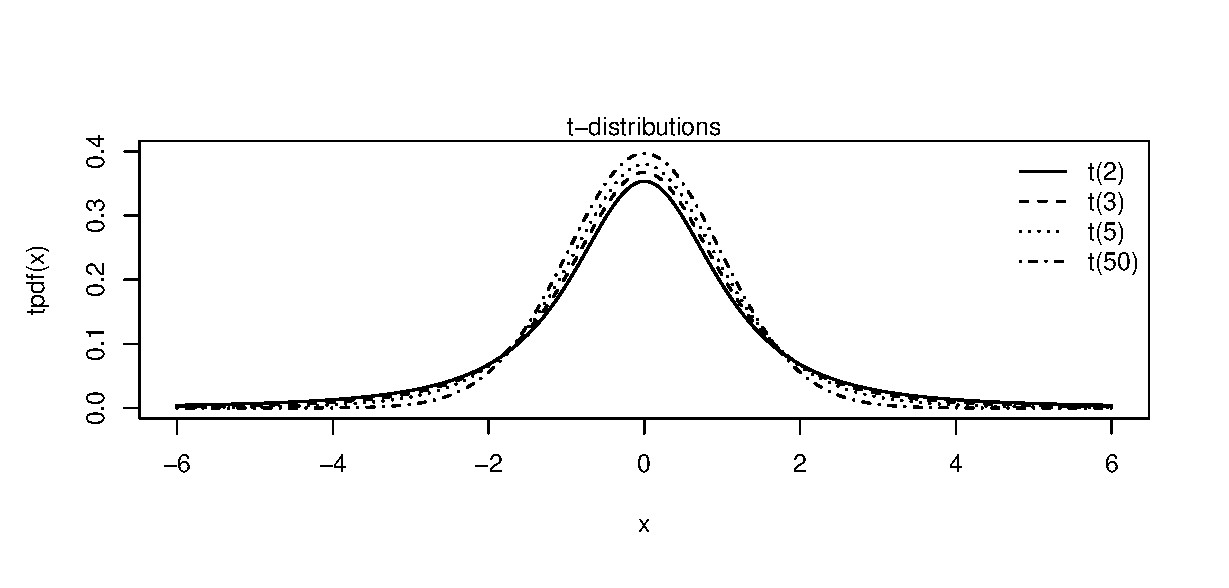
\includegraphics[scale=0.8]{tpdf.eps}
\end{center}
\caption{\texttt{pdf} of the $t$--distribution for $df=n \in \{2,
3, 5, 50\}$ degrees of freedom. For the case $t(50)$, the
$t$\texttt{pdf} is essentially equivalent to the standard
normal~\texttt{pdf}. Notice the fatter tails of the 
$t$\texttt{pdf} for small values of $n$.}
\lb{fig:tpdf}
\end{figure}
%

\medskip
\noindent
Expectation value, variance, skewness and excess kurtosis (cf. 
Rinne (2008)~\ct[p~327]{rin2008}):
%
\bea
\mathrm{E}(X) & = & 0 \\
%
\mathrm{Var}(X) & = & \frac{n}{n-2}
\quad\text{for}\quad n > 2 \\
%
\mathrm{Skew}(X) & = & 0
\quad\text{for}\quad n > 3 \\
%
\mathrm{Kurt}(X) & = & \frac{6}{n-4}
\quad\text{for}\quad n > 4 \ .
\eea
%
$\alpha$--quantiles, $t_{n;\alpha}$, of $t$--distributions, for 
which, due to the reflection symmetry of the $t$\texttt{pdf}, the 
identity $t_{n;\alpha}=-t_{n;1-\alpha}$ holds, are generally 
tabulated in textbooks on \textbf{Statistics}. Alternatively, they 
may be obtained from \R, some GDCs, EXCEL, or from OpenOffice.

\medskip
\noindent
Note that for $n \geq 50$ a $t(n)$--distribution may be 
approximated reasonably well by the standard normal distribution, 
$N(0;1)$. Again, this is a manifestation of the \textbf{central
limit theorem}, to be discussed in Sec.~\ref{sec:zentrgrenz} below.
For $n=1$, a $t(n)$--distribution amounts to a special case ($a=1$,
$b=0$) of the Cauchy distribution; cf.
Sec.~\ref{sec:cauchyverteil}.

\medskip
\noindent
\underline{\R:} $\texttt{dt}(x,n)$, $\texttt{pt}(x,n)$,
$\texttt{qt}(\alpha,n)$,
$\texttt{rt}(n_{\mathrm{simulations}},n)$ \\
\underline{GDC:} $\texttt{tpdf}(t,n)$, $\texttt{tcdf}(-10,t,n)$,
$\texttt{invT}(\alpha,n)$ \\
\underline{EXCEL, OpenOffice:} \texttt{T.DIST}, \texttt{T.INV}
(dt.: \texttt{T.VERT}, \texttt{TVERT}, \texttt{T.INV},
\texttt{TINV})

%%%%%%%%%%%%%%%%%%%%%%%%%%%%%%%%%%%%%%%%%%%%%%%%%%%%%%%%%%%%%%%%%%%
\section[$F$--distribution]{$\boldsymbol{F}$--distribution with
$n_{1}$ and $n_{2}$ degrees of freedom}
\lb{sec:fverteil}
%%%%%%%%%%%%%%%%%%%%%%%%%%%%%%%%%%%%%%%%%%%%%%%%%%%%%%%%%%%%%%%%%%%
The reproductive two-parameter
$\boldsymbol{F}$\textbf{--distribution with}
$\boldsymbol{n_{1}}$ \textbf{and} $\boldsymbol{n_{2}}$
\textbf{degrees of freedom} was made prominent in
\textbf{Statistics} by the English statistician, evolutionary
biologist, eugenicist and geneticist
\href{http://www-history.mcs.st-and.ac.uk/Biographies/Fisher.html}{Sir
Ronald Aylmer Fisher FRS (1890--1962)}, and the
US-American mathematician and statistician
\href{http://en.wikipedia.org/wiki/George_W._Snedecor}{George
Waddel Snedecor (1881--1974)}; cf. Fisher (1924)~\ct{fis1924} and 
Snedecor (1934)~\ct{sne1934}. Consider two sets of stochastically 
independent, identically standard normally distributed 
(``i.i.d.'') one-dimensional random variables, $X_{i} \sim N(0;1)$
($i=1,\ldots,n_{1}$), and $Y_{j} \sim N(0;1)$
($j=1,\ldots,n_{2}$). Define the sums
%
\be
X:=\sum_{i=1}^{n_{1}}X_{i}^{2}
\qquad\text{and}\qquad
Y:=\sum_{j=1}^{n_{2}}Y_{j}^{2} \ ,
\ee
%
each of which satisfies a $\chi^{2}$--distribution with $n_{1}$ 
resp.~$n_{2}$ degrees of freedom. Then the quotient random variable
%
\be
\fbox{$\displaystyle
F_{n_{1},n_{2}} := \frac{X/n_{1}}{Y/n_{2}} \sim F(n_{1},n_{2}) \ ,
\quad\text{with}\quad n_{1},n_{2} \in \mathbb{N} \ ,
$}
\ee
%
is $F$--distributed with $df_{1}=n_{1}$ and $df_{2}=n_{2}$ degrees 
of freedom.

\medskip
\noindent
Spectrum of values:
%
\be
F_{n_{1},n_{2}} \mapsto f_{n_{1},n_{2}}
\in D \subseteq \mathbb{R}_{\geq 0} \ .
\ee
%
The probability density function (\texttt{pdf}) of an 
$F$--distribution is quite a complicated 
mathematical expression; see Rinne (2008)~\ct[p~330]{rin2008} for
the explicit representation of the $F$\texttt{pdf}. Plots are 
shown for four different combinations of the parameters $n_{1}$ 
and $n_{2}$ in Fig.~\ref{fig:Fpdf}. The $F$\texttt{cdf}
\textit{cannot} be expressed in terms of elementary mathematical
functions.
%
\begin{figure}[!htb]
\begin{center}
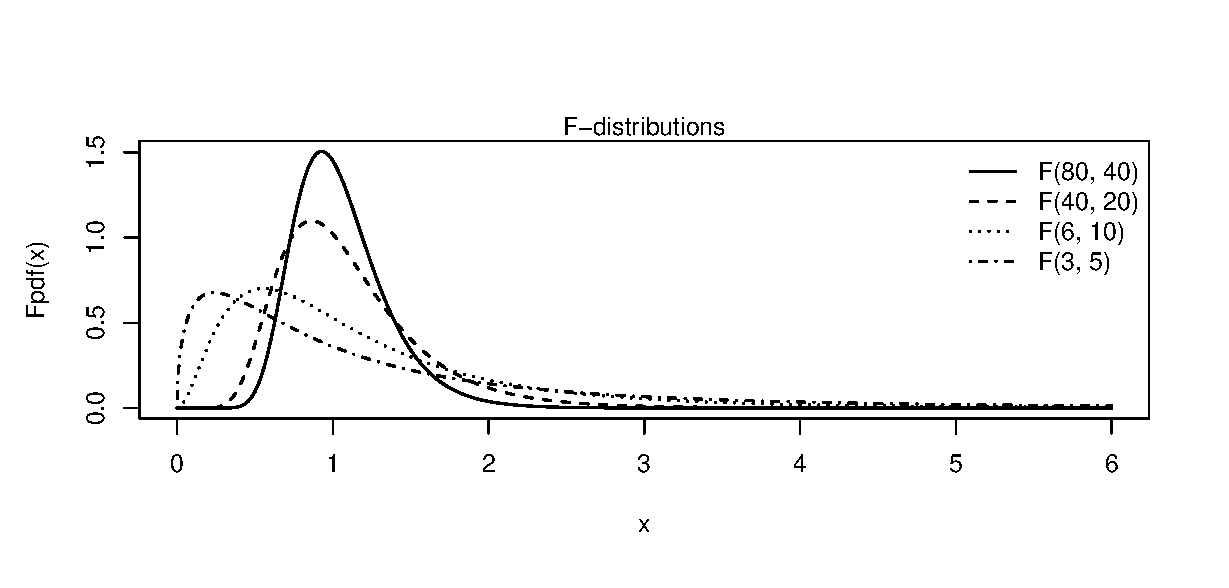
\includegraphics[scale=0.8]{Fpdf.eps}
\end{center}
\caption{\texttt{pdf} of the $F$--distribution for four
combinations of degrees of freedom $(df_{1}=n_{1}, df_{2}=n_{2})$.
The curves correspond to the cases $F(80,40)$, $F(40,20)$,
$F(6,10)$ and $F(3,5)$, respectively.}
\lb{fig:Fpdf}
\end{figure}
%

\medskip
\noindent
Expectation value, variance, skewness and excess kurtosis (cf. 
Rinne (2008)~\ct[p~332]{rin2008}):
%
\bea
\mathrm{E}(X) & = & \frac{n_{2}}{n_{2}-2} \quad\text{for}\quad
n_{2} > 2\\
%
\mathrm{Var}(X) & = & \frac{2n_{2}^{2}(n_{1}+n_{2}-2)}{
n_{1}(n_{2}-2)^{2}(n_{2}-4)}
\quad\text{for}\quad n_{2} > 4 \\
%
\mathrm{Skew}(X) & = & \frac{(2n_{1}+n_{2}-2)\sqrt{8(n_{2}-4)}}{
(n_{2}-6)\sqrt{n_{1}(n_{1}+n_{2}-2)}}
\quad\text{for}\quad n_{2} > 6 \\
%
\mathrm{Kurt}(X) & = & 
12\,\frac{n_{1}(5n_{2}-22)(n_{1}+n_{2}-2)+(n_{2}-2)^{2}(n_{2}-4)}{
n_{1}(n_{2}-6)(n_{2}-8)(n_{1}+n_{2}-2)}
\quad\text{for}\quad n_{2} > 8 \ .
\eea
%
$\alpha$--quantiles, $f_{n_{1},n_{2};\alpha}$, of 
$F$--distributions are tabulated in advanced textbooks on 
\textbf{Statistics}. Alternatively, they may be obtained from \R,
EXCEL, or from OpenOffice.

\medskip
\noindent
\underline{\R:} $\texttt{df}(x,n_{1}, n_{2})$,
$\texttt{pf}(x,n_{1}, n_{2})$, $\texttt{qf}(\alpha,n_{1}, n_{2})$,
$\texttt{rf}(n_{\mathrm{simulations}},n_{1}, n_{2})$ \\
\underline{GDC:} $F\texttt{pdf}(x,n_{1},n_{2})$,
$F\texttt{cdf}(0,x,n_{1},n_{2})$ \\
\underline{EXCEL, OpenOffice:} \texttt{F.DIST}, \texttt{F.INV}
(dt.: \texttt{F.VERT}, \texttt{FVERT}, \texttt{F.INV},
\texttt{FINV})

%%%%%%%%%%%%%%%%%%%%%%%%%%%%%%%%%%%%%%%%%%%%%%%%%%%%%%%%%%%%%%%%%%%
\section[Pareto distribution]{Pareto distribution}
\lb{sec:paretodistr}
%%%%%%%%%%%%%%%%%%%%%%%%%%%%%%%%%%%%%%%%%%%%%%%%%%%%%%%%%%%%%%%%%%%
When studying the distribution of wealth and income of people in 
Italy towards the end of the $19^\mathrm{th}$ Century, the Italian 
engineer, sociologist, economist, political scientist and 
philosopher
\href{http://en.wikipedia.org/wiki/Vilfredo_Pareto}{Vilfredo
Federico Damaso Pareto (1848--1923)} discovered a certain type of 
quantitative regularity which he could model mathematically in 
terms of a simple power-law function involving only two free 
parameters; cf. Pareto (1896)~\ct{par1896}. The one-dimensional 
random variable~$X$ underlying such a \textbf{Pareto distribution},
%
\be
X \sim Par(\gamma,x_\mathrm{min}) \ ,
\ee
%
has a

\medskip
\noindent
Spectrum of values:
%
\be
X \mapsto x \in \{x|x \geq x_\mathrm{min}\} \subset \mathbb{R}_{>0}
\ ,
\ee
%
and a

\medskip
\noindent
Probability density function (\texttt{pdf}):
%
\be
\lb{paretopdf}
\fbox{$\displaystyle
f_{X}(x)=
\begin{cases}
0 & \text{for}\quad x < x_\mathrm{min} \\
\\
{\displaystyle \frac{\gamma}{x_\mathrm{min}}
\left(\frac{x_\mathrm{min}}{x}\right)^{\gamma+1}} \ ,
\quad \gamma \in \mathbb{R}_{>0}
& \text{for}\quad x \geq x_\mathrm{min}
\end{cases} \ ;
$}
\ee
%
%
its graph is shown in Fig.~\ref{fig:parpdf} below for four 
different values of the dimensionless exponent~$\gamma$.
%
\begin{figure}[!htb]
\begin{center}
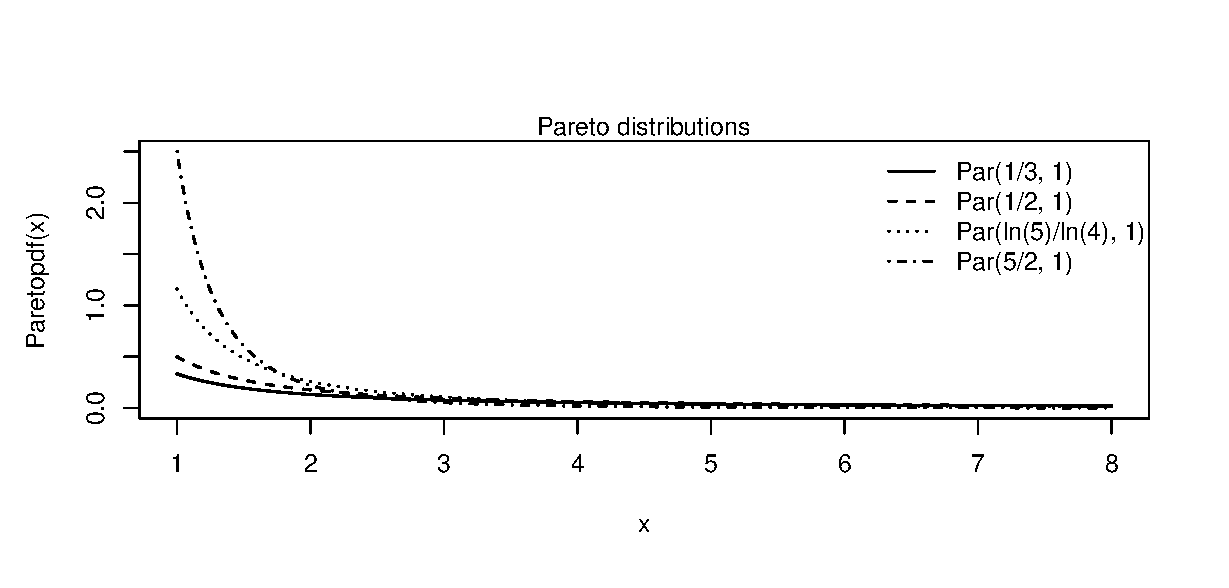
\includegraphics[scale=0.8]{parpdf.eps}
\end{center}
\caption{\texttt{pdf} of the Pareto distribution according 
to Eq.~(\ref{paretopdf}) for $x_\mathrm{min}=1$ and $\displaystyle 
\gamma \in \left\{\frac{1}{3}, \frac{1}{2}, \frac{\ln(5)}{\ln(4)}, 
\frac{5}{2}\right\}$.}
\lb{fig:parpdf}
\end{figure}
%

\medskip
\noindent
Cumulative distribution function (\texttt{cdf}):
%
\be
\fbox{$\displaystyle
F_{X}(x) = P(X \leq x)
=
\begin{cases}
0 & \text{for}\quad x < x_\mathrm{min} \\
\\
{\displaystyle 1-\left(\frac{x_\mathrm{min}}{x}\right)^{\gamma}}
& \text{for}\quad x \geq x_\mathrm{min}
\end{cases} \ .
$}
\lb{paretocdf}
\ee
%
Expectation value, variance, skewness and excess kurtosis (cf. 
Rinne (2008)~\ct[p~362]{rin2008}):
%
\bea
\mathrm{E}(X) & = & \frac{\gamma}{\gamma-1}\,x_\mathrm{min}
\qquad\text{for}\quad \gamma > 1 \\
%
\lb{eq:paretovar}
\mathrm{Var}(X) & = & \frac{\gamma}{(\gamma-1)^{2}(\gamma-2)}\,
x_\mathrm{min}^{2}
\qquad\text{for}\quad \gamma > 2 \\
%
\mathrm{Skew}(X) & = & 
\frac{2(1+\gamma)}{\gamma-3}\,\sqrt{\frac{\gamma-2}{\gamma}}
\qquad\text{for}\quad \gamma > 3 \\
%
\mathrm{Kurt}(X) & = & 
\frac{6(\gamma^{3}+\gamma^{2}-6\gamma-2)}{\gamma(\gamma-3)
(\gamma-4)}
\qquad\text{for}\quad \gamma > 4 \ .
\eea
%
It is important to realise that $\mathrm{E}(X)$, $\mathrm{Var}(X)$, 
$\mathrm{Skew}(X)$ and $\mathrm{Kurt}(X)$ are \textit{well-defined
only} for the values of $\gamma$ indicated; otherwise these
measures do not exist.

\medskip
\noindent
$\alpha$--quantiles:
%
\be
\lb{alphapareto}
\alpha \stackrel{!}{=} F_{X}(x_{\alpha})
= 1-\left(\frac{x_\mathrm{min}}{x_{\alpha}}\right)^{\gamma}
\ \Leftrightarrow\ 
x_{\alpha} = F_{X}^{-1}(\alpha)
= \sqrt[\gamma]{\frac{1}{1-\alpha}}\,x_\mathrm{min}
\quad\text{for\ all}\quad 0 < \alpha < 1 \ .
\ee
%

\medskip
\noindent
\underline{\R:}
$\texttt{dpareto}(x, \gamma, x_{\mathrm{min}})$,
$\texttt{ppareto}(x, \gamma, x_{\mathrm{min}})$,
$\texttt{qpareto}(\alpha, \gamma, x_{\mathrm{min}})$, \\
$\texttt{rpareto}(n_{\mathrm{simulations}}, \gamma,
x_{\mathrm{min}})$ (package: {\tt extraDistr}, by Wolodzko
(2018)~\ct{wol2018})

\medskip
\noindent
Note that it follows from Eq.~(\ref{paretocdf}) that the 
probability of a Pareto-distributed continuous one-dimensional 
random variable $X$ to exceed a certain threshold value $x$ is 
given by the simple power-law rule
%
\be
P(X > x)
= 1 - P(X \leq x)
= \left(\frac{x_\mathrm{min}}{x}\right)^{\gamma} \ .
\ee
%
Hence, the ratio of probabilities
%
\be
\frac{P(X>kx)}{P(X>x)}
=\frac{{\displaystyle \left(\frac{x_\mathrm{min}}{kx}
\right)^{\gamma}}}{{\displaystyle
\left(\frac{x_\mathrm{min}}{x}\right)^{\gamma}}}
= \left(\frac{1}{k}\right)^{\gamma} \ ,
\ee
%
with $k \in \mathbb{R}_{>0}$, is \textbf{scale-invariant}, meaning
independent of a particular scale $x$ at which one observes $X$ 
(cf. Taleb (2007)~\ct[p~256ff and p~326ff]{tal2007}). This 
behaviour is a direct consequence of a special mathematical 
property of Pareto distributions which is technically referred to 
as \textbf{self-similarity}. It is determined by the fact that 
a Pareto--\texttt{pdf} (\ref{paretopdf}) has \textit{constant}
elasticity, i.e. (cf. Ref.~\ct[Sec.~7.6]{hve2009})
%
\be
\varepsilon_{f_{X}}(x) = -(\gamma+1)
\quad\text{for}\quad x \geq x_\mathrm{min} \ ,
\ee
%
which contrasts with the case of the standard normal 
distribution; cf. Eq.~(\ref{eq:phielasts}). This feature implies
that in the present scenario the occurrence of extreme
\textbf{outliers} for~$X$ is not entirely unusual.

\medskip
\noindent
Further interesting examples, in various fields of applied science,
of distributions of quantities which also feature the 
scale-invariance of scaling laws are described in 
Wiesenfeld (2001)~\ct{wie2001}. Nowadays, Pareto distributions 
play an important role in the quantitative modelling of financial 
risk; see, e.g., Bouchaud and Potters (2003)~\ct{boupot2003}.

\medskip
\noindent
Working out the equation of the Lorenz curve associated with a 
Pareto distribution according to Eq.~(\ref{lorcurve}), using
Eq.~(\ref{alphapareto}), yields a particularly simple result
given by
%
\be
L(\alpha;\gamma) = 1 - (1-\alpha)^{1-(1/\gamma)} \ .
\ee
%
This result forms the basis of Pareto's famous \textbf{80/20 rule} 
concerning concentration in the distribution of various assets of 
general importance in a given population. According to Pareto's 
empirical findings, typically 80\% of such an asset are owned by 
just 20\% of the population considered (and vice versa); cf. 
Pareto (1896)~\ct{par1896}.\footnote{See also footnote 2 in 
Sec.~\ref{subsec:gini}.} The 80/20 rule applies exactly for a 
value of the power-law index of ${\displaystyle\gamma = 
\frac{\ln(5)}{\ln(4)}} \approx 1.16$. It is a prominent example of 
the phenomenon of \textbf{universality}, frequently observed in the 
mathematical modelling of quantitative--empirical relationships 
between variables in a wide variety of scientific disciplines; cf. 
Gleick (1987)~\ct[p~157ff]{gle1987}.

\medskip
\noindent
For purposes of numerical simulation it is useful to work with a 
\textbf{truncated Pareto distribution}, for which the
one-dimensional random variable~$X$ takes values in an interval
$\left[x_\mathrm{min},x_\mathrm{cut}\right] \subset
\mathbb{R}_{>0}$. Samples of 
random values for such an $X$ can be easily generated from a 
one-dimensional random variable $Y$ that is uniformly distributed 
on the interval $\left[0,1\right]$. The sample values of the latter
are subsequently transformed according to the formula; cf. 
Ref.~\ct{wol2015}:
%
\be
x(y) = \frac{x_\mathrm{min}x_\mathrm{cut}}{\left[x_\mathrm{
cut}^{\gamma}-\left(x_\mathrm{cut}^{\gamma}-x_\mathrm{
min}^{\gamma}\right)y\right]^{1/\gamma}} \ .
\ee
%
The required uniformly distributed random numbers $y \in 
\left[0,1\right]$ can be obtained, e.g., from \R\ by means of
$\texttt{runif}(n_{\mathrm{simulations}},0,1)$, or from the random
number generator \texttt{RAND()} (dt.: \texttt{ZUFALLSZAHL()})
in EXCEL or in OpenOffice.

\leftout{
%%%%%%%%%%%%%%%%%%%%%%%%%%%%%%%%%%%%%%%%%%%%%%%%%%%%%%%%%%%%%%%%%%%
\section[Power-law distribution]{Power-law distribution}
\lb{sec:powerlawdistr}
%%%%%%%%%%%%%%%%%%%%%%%%%%%%%%%%%%%%%%%%%%%%%%%%%%%%%%%%%%%%%%%%%%%
While the \texttt{pdf} of a Pareto distribution, discussed in the 
previous section, is proportional to positive powers of $1/x$, the 
slightly more general three-parameter \textbf{power-law distribution},
%
\be
X \sim Pl(a;b;c) \ .
\ee
%
includes cases with a \texttt{pdf} proportional to positive 
powers of $x$ itself (i.e., for $c>1$).

\medskip
\noindent
Spectrum of values:
%
\be
X \mapsto x \in \{x|a \leq x \leq a+b, b \in \mathbb{R}_{>0}\}
\subset \mathbb{R} \ .
\ee
%
Probability density function (\texttt{pdf}):
%
\be
\lb{powerlawpdf}
\fbox{$\displaystyle
f_{X}(x) =
\begin{cases}
0 & \text{for}\quad x < a \\ \\
{\displaystyle \frac{c}{b}\left(\frac{x-a}{b}\right)^{c-1}} \ ,
\quad c \in \mathbb{R}_{>0}
& \text{for}\quad a \leq x \leq a+b \\ \\
0 & \text{for}\quad x > b
\end{cases} \ .
$}
\ee
%
Cumulative distribution function (\texttt{cdf}):
%
\be
\lb{powerlawcdf}
\fbox{$\displaystyle
F_{X}(x) = P(X \leq x)
=
\begin{cases}
0 & \text{for}\quad x < a \\ \\
{\displaystyle \left(\frac{x-a}{b}\right)^{c}}
& \text{for}\quad a \leq x \leq a+b \\ \\
1 & \text{for}\quad x > b
\end{cases} \ .
$}
\ee
%
Expectation value and variance:
%
\bea
\mathrm{E}(X) & = & a + \frac{c}{c+1}\,b \\
\mathrm{Var}(X) & = & \frac{c}{(c+1)^{2}(c+2)}\,b^{2} \ .
\eea
%
$\alpha$--quantiles:
%
\be
\alpha \stackrel{!}{=} F_{X}(x_{\alpha})
= \left(\frac{x_{\alpha}-a}{b}\right)^{c}
\ \Leftrightarrow\ 
x_{\alpha} = F_{X}^{-1}(\alpha)
= a + \sqrt[c]{\alpha}\times b
\quad\text{for\ all}\quad 0 < \alpha < 1 \ .
\ee
%
}

%%%%%%%%%%%%%%%%%%%%%%%%%%%%%%%%%%%%%%%%%%%%%%%%%%%%%%%%%%%%%%%%%%%
\section[Exponential distribution]{Exponential distribution}
\lb{sec:expdistr}
%%%%%%%%%%%%%%%%%%%%%%%%%%%%%%%%%%%%%%%%%%%%%%%%%%%%%%%%%%%%%%%%%%%
The \textbf{exponential distribution} for a continuous 
one-dimensional random variable $X$,
%
\be
X \sim Ex(\lambda) \ ,
\ee
%
depends on a single free parameter, $\lambda \in \mathbb{R}_{>0}$, 
which represents an inverse scale.

\medskip
\noindent
Spectrum of values:
%
\be
X \mapsto x \in \mathbb{R}_{\geq 0} \ .
\ee
%
Probability density function (\texttt{pdf}):
%
\be
\lb{eq:exppdf}
\fbox{$\displaystyle
f_{X}(x) = 
\begin{cases}
0 &
\text{for}\quad x < 0 \\ \\
\lambda\exp\left[-\lambda x\right]  \ ,
\quad \lambda \in \mathbb{R}_{>0} &
\text{for}\quad x \geq 0
\end{cases} \ ;
$}
\ee
%
its graph is shown in Fig.~\ref{fig:exppdf} below.
%
\begin{figure}[!htb]
\begin{center}
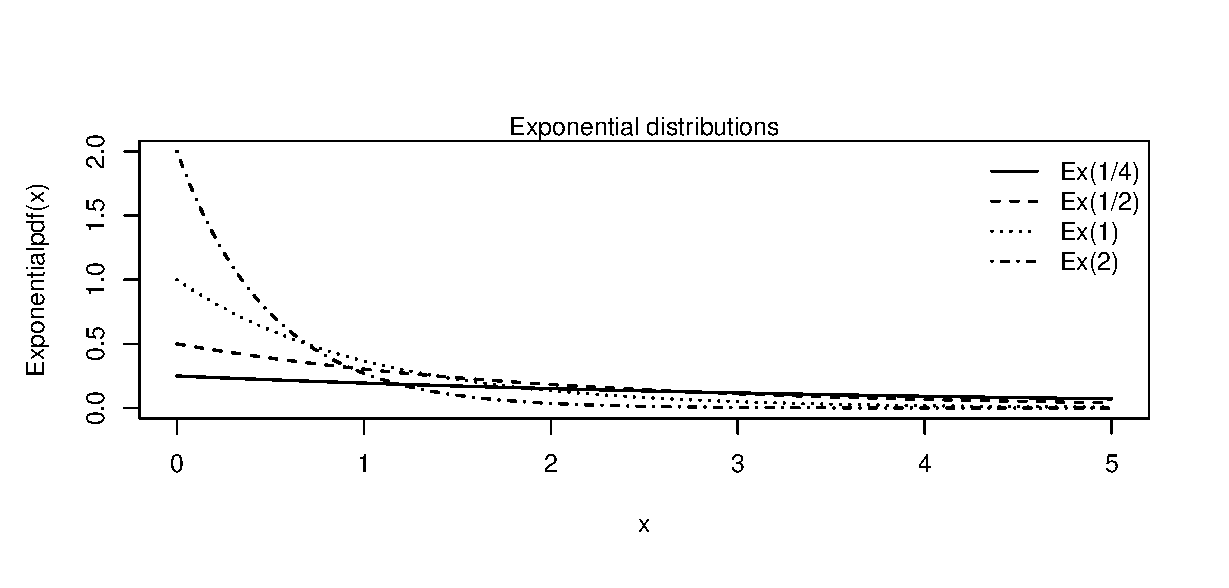
\includegraphics[scale=0.8]{exppdf.eps}
\end{center}
\caption{\texttt{pdf} of the exponential distribution 
according to Eq.~(\ref{eq:exppdf}). Displayed are the cases 
$Ex(1/4)$, $Ex(1/2)$, $Ex(1)$ and $Ex(2)$.}
\lb{fig:exppdf}
\end{figure}
%

\medskip
\noindent
Cumulative distribution function (\texttt{cdf}):
%
\be
\fbox{$\displaystyle
F_{X}(x) = P(X \leq x)
=
\begin{cases}
0 & \text{for}\quad x < 0 \\ \\
1 - \exp\left[-\lambda x\right] &
\text{for}\quad x \geq 0
\end{cases} \ .
$}
\ee
%
Expectation value, variance, skewness and excess 
kurtosis:\footnote{The derivation of these results entails 
integration by parts for a number of times; see, e.g., 
Ref.~\ct[Sec.~8.1]{hve2009}.}
%
\bea
\mathrm{E}(X) & = & \frac{1}{\lambda} \\
%
\mathrm{Var}(X) & = & \frac{1}{\lambda^{2}} \\
%
\mathrm{Skew}(X) & = & 2 \\
%
\mathrm{Kurt}(X) & = & 6 \ .
\eea
%
$\alpha$--quantiles:
%
\be
\alpha \stackrel{!}{=} F_{X}(x_{\alpha})
= 1 - \exp\left[-\lambda x_{\alpha}\right]
\ \Leftrightarrow\ 
x_{\alpha} = F_{X}^{-1}(\alpha)
= -\,\frac{\ln(1-\alpha)}{\lambda}
\quad\text{for\ all}\quad 0 < \alpha < 1 \ .
\ee
%

\medskip
\noindent
\underline{\R:} $\texttt{dexp}(x,\lambda)$,
$\texttt{pexp}(x,\lambda)$, $\texttt{qexp}(\alpha,\lambda)$,
$\texttt{rexp}(n_{\mathrm{simulations}},\lambda)$

%%%%%%%%%%%%%%%%%%%%%%%%%%%%%%%%%%%%%%%%%%%%%%%%%%%%%%%%%%%%%%%%%%%
\section[Logistic distribution]{Logistic distribution}
\lb{sec:logisticdistr}
%%%%%%%%%%%%%%%%%%%%%%%%%%%%%%%%%%%%%%%%%%%%%%%%%%%%%%%%%%%%%%%%%%%
The \textbf{logistic distribution} for a continuous one-dimensional 
random variable $X$,
%
\be
X \sim Lo(\mu;s) \ ,
\ee
%
depends on two free parameters: a location parameter $\mu \in \mathbb{R}$ and a scale parameter $s \in \mathbb{R}_{>0}$.

\medskip
\noindent
Spectrum of values:
%
\be
X \mapsto x \in \mathbb{R} \ .
\ee
%
Probability density function (\texttt{pdf}):
%
\be
\lb{eq:logisticpdf}
\fbox{$\displaystyle
f_{X}(x) = \frac{\exp\left[{\displaystyle 
-\frac{x-\mu}{s}}\right]}{s\left(1+
\exp\left[{\displaystyle -\frac{x-\mu}{s}}\right]\right)^{2}} \ ,
\quad \mu \in\mathbb{R}\ , s \in \mathbb{R}_{>0} \ ;
$}
\ee
%
its graph is shown in Fig.~\ref{fig:logisticpdf} below.
%
\begin{figure}[!htb]
\begin{center}
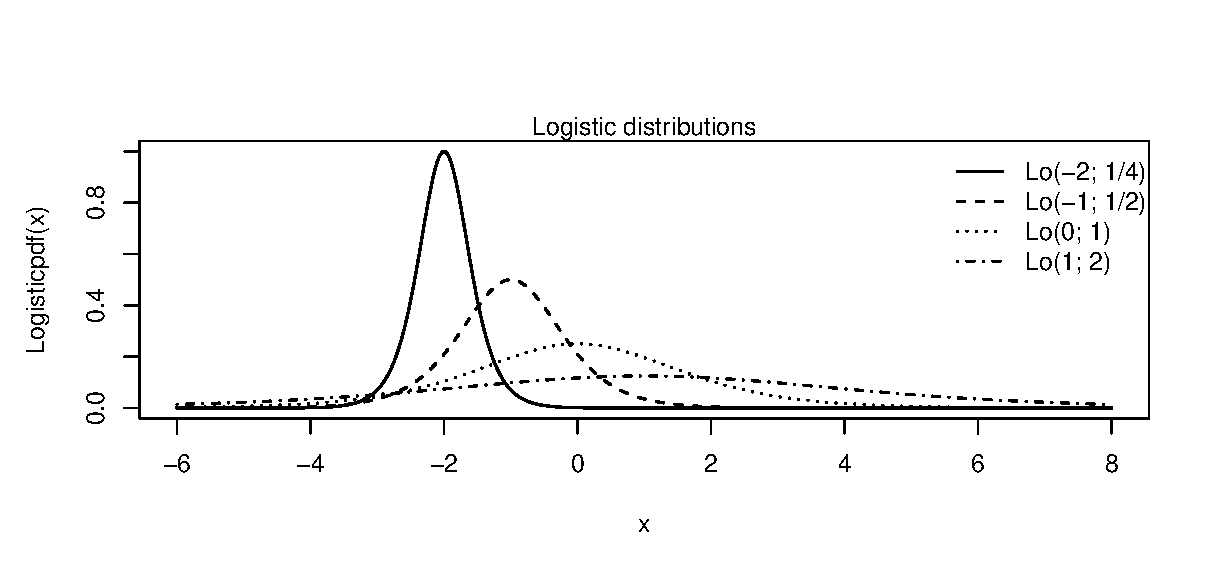
\includegraphics[scale=0.8]{logisticpdf.eps}
\end{center}
\caption{\texttt{pdf} of the logistic distribution 
according to Eq.~(\ref{eq:logisticpdf}). Displayed are the cases 
$Lo(-2;1/4)$, $Lo(-1;1/2)$, $Lo(0;1)$ and $Lo(1;2)$.}
\lb{fig:logisticpdf}
\end{figure}
%

\medskip
\noindent
Cumulative distribution function (\texttt{cdf}):
%
\be
\fbox{$\displaystyle
F_{X}(x) = P(X \leq x)
= \frac{1}{1+\exp\left[{\displaystyle -\frac{x-\mu}{s}}\right]} \ .
$}
\ee
%
Expectation value, variance, skewness and excess kurtosis (cf. 
Rinne (2008)~\ct[p~359]{rin2008}):
%
\bea
\mathrm{E}(X) & = & \mu \\
%
\mathrm{Var}(X) & = & \frac{s^{2}\pi^{2}}{3} \\
%
\mathrm{Skew}(X) & = & 0 \\
%
\mathrm{Kurt}(X) & = & \frac{6}{5} \ .
\eea
%
$\alpha$--quantiles:
%
\be
\alpha \stackrel{!}{=} F_{X}(x_{\alpha})
= \frac{1}{1+\exp\left[{\displaystyle 
-\frac{x_{\alpha}-\mu}{s}}\right]}
\ \Leftrightarrow\ 
x_{\alpha} = F_{X}^{-1}(\alpha)
= \mu + s\ln\left(\frac{\alpha}{1-\alpha}\right)
\quad\text{for\ all}\quad 0 < \alpha < 1 \ .
\ee
%

\medskip
\noindent
\underline{\R:} $\texttt{dlogis}(x,\mu,s)$,
$\texttt{plogis}(x,\mu,s)$, $\texttt{qlogis}(\alpha,\mu,s)$,
$\texttt{rlogis}(n_{\mathrm{simulations}},\mu,s)$

%%%%%%%%%%%%%%%%%%%%%%%%%%%%%%%%%%%%%%%%%%%%%%%%%%%%%%%%%%%%%%%%%%%
\section[Special hyperbolic distribution]{Special hyperbolic
distribution}
\lb{sec:hyperbelverteil}
%%%%%%%%%%%%%%%%%%%%%%%%%%%%%%%%%%%%%%%%%%%%%%%%%%%%%%%%%%%%%%%%%%%
The complex dynamics associated with the formation of generic 
singularities in relativistic cosmology can be perceived as a 
random process. In this context, the following \textbf{special 
hyperbolic distribution} for a continuous one-dimensional random 
variable $X$,
%
\be
X \sim sHyp \ ,
\ee
%
which does not depend on any free parameters, was introduced by 
Khalatnikov {\em et al\/} (1985)~\ct{khaetal1985} to aid a 
simplified dynamical description of singularity formation; see 
also Heinzle {\em et al\/} (2009)~\ct[Eq.~(50)]{heietal2009}.

\medskip
\noindent
Spectrum of values:
%
\be
X \mapsto x \in \left[0,1\right]
\subset \mathbb{R}_{\geq 0} \ .
\ee
%
Probability density function (\texttt{pdf}):
%
\be
\lb{eq:sHyppdf}
\fbox{$\displaystyle
f_{X}(x) = 
\begin{cases}
{\displaystyle \frac{1}{\ln(2)}\,\frac{1}{1+x}} &
\text{for}\quad x \in \left[0,1\right] \\ \\
0 & \text{otherwise}
\end{cases} \ ;
$}
\ee
%
its graph is shown in Fig.~\ref{fig:sHyppdf} below.
%
\begin{figure}[!htb]
\begin{center}
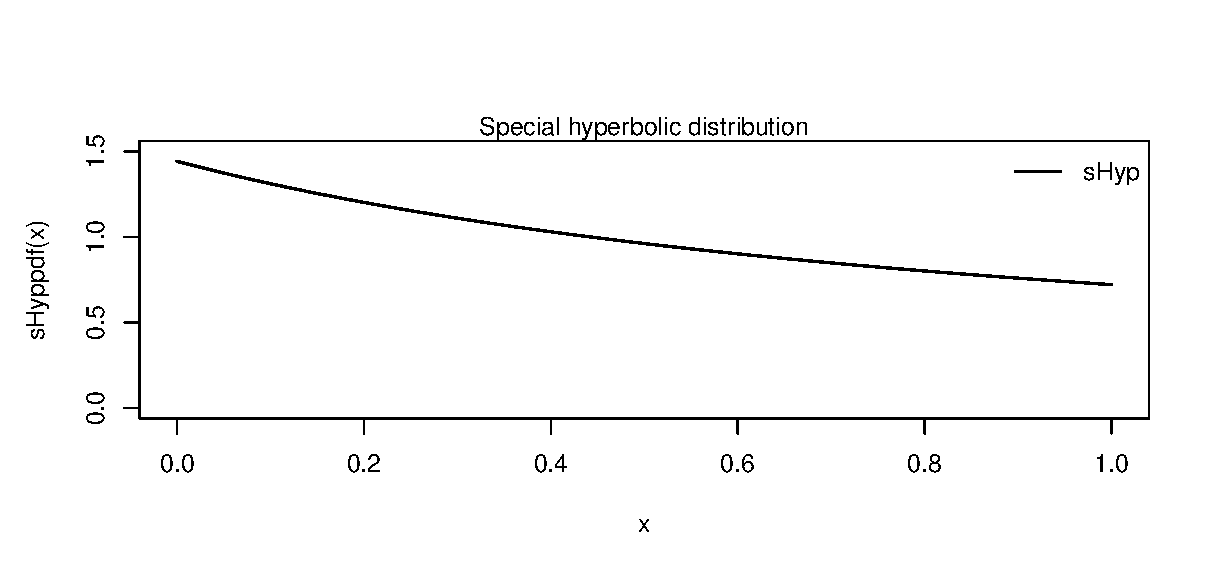
\includegraphics[scale=0.8]{sHyppdf.eps}
\end{center}
\caption{\texttt{pdf} of the special hyperbolic distribution 
according to Eq.~(\ref{eq:sHyppdf}).}
\lb{fig:sHyppdf}
\end{figure}
%

\medskip
\noindent
Cumulative distribution function (\texttt{cdf}):
%
\be
\fbox{$\displaystyle
F_{X}(x) = P(X \leq x)
=
\begin{cases}
0 & \text{for}\quad x < 0 \\ \\
{\displaystyle \frac{1}{\ln(2)}\,\ln(1+x)} &
\text{for}\quad x \in \left[0,1\right] \\ \\
1 & \text{for}\quad x > 1
\end{cases} \ .
$}
\ee
%
Expectation value, variance, skewness and excess 
kurtosis:\footnote{Use polynomial division to simplify the 
integrands in the ensuing moment integrals when verifying these 
results.}
%
\bea
% Results for Skew(X) and Kurt(X) derived on Do, 15.8.2013; these 
% require conformation.
\mathrm{E}(X) & = & \frac{1-\ln(2)}{\ln(2)} \\
%
\mathrm{Var}(X) & = & \frac{3\ln(2)-2}{2\left[
\ln(2)\right]^{2}} \\
%
\mathrm{Skew}(X) & = & \frac{7\left[
\ln(2)\right]^{2}-\frac{27}{2}\ln(2)+6}{3\left(\frac{1}{2}
\right)^{3/2}\left[3\ln(2)-2\right]^{3/2}} \\
%
\mathrm{Kurt}(X) & = & \frac{15\left[
\ln(2)\right]^{3}-\frac{193}{3}\left[
\ln(2)\right]^{2}+72\ln(2)-24}{\left[
3\ln(2)-2\right]^{2}} \ .
\eea
%
$\alpha$--quantiles:
%
\be
\alpha \stackrel{!}{=} F_{X}(x_{\alpha})
= \frac{1}{\ln(2)}\,\ln(1+x_{\alpha})
\ \Leftrightarrow\ 
x_{\alpha} = F_{X}^{-1}(\alpha)
= e^{\alpha\ln(2)}-1
\quad\text{for\ all}\quad 0 < \alpha < 1 \ .
\ee
%

%%%%%%%%%%%%%%%%%%%%%%%%%%%%%%%%%%%%%%%%%%%%%%%%%%%%%%%%%%%%%%%%%%%
\section[Cauchy distribution]{Cauchy distribution}
\lb{sec:cauchyverteil}
%%%%%%%%%%%%%%%%%%%%%%%%%%%%%%%%%%%%%%%%%%%%%%%%%%%%%%%%%%%%%%%%%%%
The French mathematician
\href{http://www-history.mcs.st-and.ac.uk/Biographies/Cauchy.html} {Augustin Louis Cauchy (1789--1857)} is credited with the inception into
\textbf{Statistics} of the continuous two-parameter 
distribution law
%
\be
X \sim Ca(b;a) \ ,
\ee
%
with properties

\medskip
\noindent
Spectrum of values:
%
\be
X \mapsto x \in \mathbb{R} \ .
\ee
%
Probability density function (\texttt{pdf}):
%
\be
\lb{cauchypdf}
\fbox{$\displaystyle
f_{X}(x) = \frac{1}{\pi}\,\frac{a}{a^{2}+(x-b)^{2}} \ ,
\qquad\text{with}\quad a \in \mathbb{R}_{>0},\ b \in \mathbb{R} \ ;
$}
\ee
%
its graph is shown in Fig.~\ref{fig:capdf} below for two 
particular cases.
%
\begin{figure}[!htb]
\begin{center}
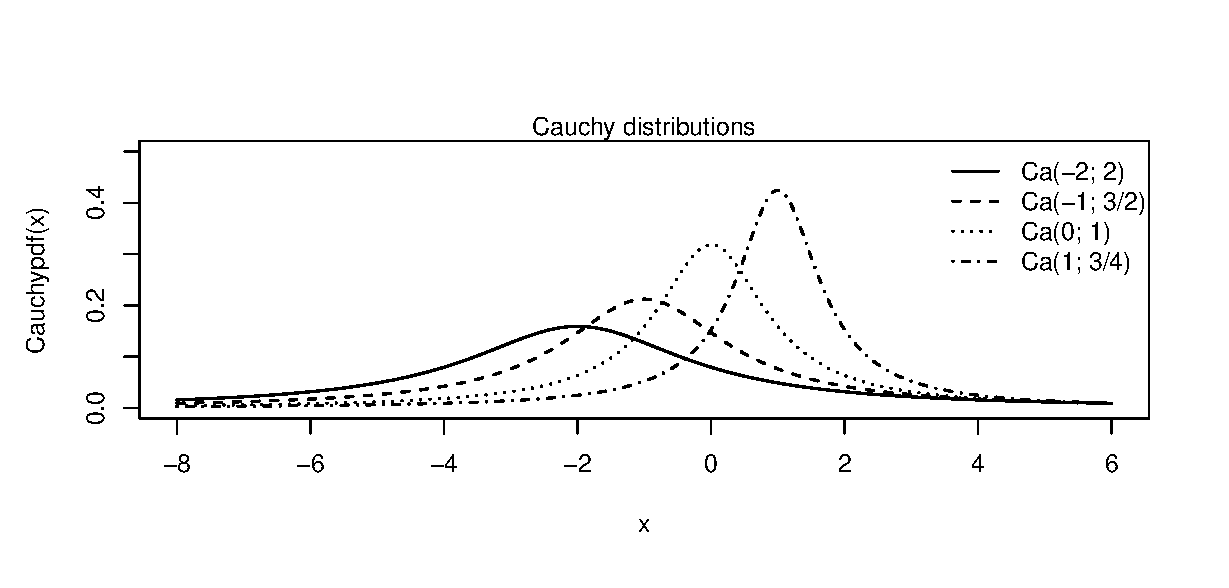
\includegraphics[scale=0.8]{capdf.eps}
\end{center}
\caption{\texttt{pdf} of the Cauchy distribution according to 
Eq.~(\ref{cauchypdf}). Displayed are the cases $Ca(-2;2)$,
$Ca(-1;3/2)$, $Ca(0;1)$ and $Ca(1;3/4)$. The case $Ca(0;1)$
corresponds to a $t$--distribution with $df = 1$ degree of freedom;
cf. Sec.~\ref{sec:tverteil}.}
\lb{fig:capdf}
\end{figure}
%

\medskip
\noindent
Cumulative distribution function (\texttt{cdf}):
%
\be
\lb{cauchycdf}
\fbox{$\displaystyle
F_{X}(x) = P(X \leq x)
= \frac{1}{2}
+ \frac{1}{\pi}\,\arctan\left(\frac{x-b}{a}\right) \ .
$}
\ee
%
Expectation value, variance, skewness and excess 
kurtosis:\footnote{In the case of a Cauchy distribution the 
fall-off in the tails of the \texttt{pdf} is not sufficiently fast 
for the expectation value and variance integrals, 
Eqs.~(\ref{eq:expectcon}) and (\ref{eq:varcon}), to 
converge to finite values. Consequently, this also concerns the 
skewness and excess kurtosis given in Eqs.~(\ref{eq:skew2}) and 
(\ref{eq:kurt2}).}
%
\bea
\mathrm{E}(X): & \quad & \text{does NOT exist due to a
diverging integral} \\
%
\mathrm{Var}(X): & \quad & \text{does NOT exist due to a
diverging integral} \\
%
\mathrm{Skew}(X): & \quad & \text{does NOT exist due to a
diverging integral} \\
%
\mathrm{Kurt}(X): & \quad & \text{does NOT exist due to a
diverging integral} \ .
\eea
%
See, e.g., Sivia and Skilling (2006) \ct[p~34]{sivski2006}.

\medskip
\noindent
$\alpha$--quantiles:
%
\be
\alpha \stackrel{!}{=} F_{X}(x_{\alpha})
\quad\Leftrightarrow\quad
x_{\alpha} = F_{X}^{-1}(\alpha)
= b + a\tan\left[\pi\left(\alpha-\frac{1}{2}\right)\right]
\quad\text{for\ all}\quad 0 < \alpha < 1 \ .
\ee
%

\medskip
\noindent
\underline{\R:} $\texttt{dcauchy}(x,b,a)$,
$\texttt{pcauchy}(x,b,a)$, $\texttt{qcauchy}(\alpha,b,a)$,
$\texttt{rcauchy}(n_{\mathrm{simulations}},b,a)$

%%%%%%%%%%%%%%%%%%%%%%%%%%%%%%%%%%%%%%%%%%%%%%%%%%%%%%%%%%%%%%%%%%%
\section[Central limit theorem]{Central limit theorem}
\lb{sec:zentrgrenz}
%%%%%%%%%%%%%%%%%%%%%%%%%%%%%%%%%%%%%%%%%%%%%%%%%%%%%%%%%%%%%%%%%%%
The first systematic derivation and presentation of the paramount
\textbf{central limit theorem} of \textbf{Probability Theory} is
due to the French mathematician and astronomer 
\href{http://www-history.mcs.st-and.ac.uk/Biographies/Laplace.html}{Marquis Pierre Simon de Laplace (1749--1827)}, cf. Laplace 
(1809)~\ct{lap1809}.

\medskip
\noindent
Consider a set of $n$ \textbf{mutually stochastically independent} 
[cf. Eqs.~(\ref{eq:stochindep2}) and~(\ref{eq:stochindep3})],
\textbf{additive} one-dimensional random variables
$X_{1},\ldots, X_{n}$, with
%
\begin{itemize}

\item[(i)] \textit{finite} expectation values 
$\mu_{1}, \ldots, \mu_{n}$,

\item[(ii)] \textit{finite} variances 
$\sigma_{1}^{2}, \ldots, \sigma_{n}^{2}$,
which are not too different from one another, and 

\item[(iii)] corresponding \texttt{cdf}s 
$F_{1}(x), \ldots, F_{n}(x)$.
\end{itemize}
%
Introduce for this set a \textbf{total sum}~$Y_{n}$ according to 
Eq.~(\ref{eq:sumnmean}), and, by standardisation 
via~Eq.~(\ref{eq:standardisation}), a related \textbf{standardised 
summation random variable}
%
\be
\displaystyle
Z_{n} := 
\frac{Y_{n}-{\displaystyle\sum_{i=1}^{n}\mu_{i}}}{\sqrt{{\displaystyle\sum_{j=1}^{n}\sigma_{j}^{2}}}} \ .
\ee
%
Let ${\cal F}_{n}(z_{n})$ denote the \texttt{cdf} associated with
$Z_{n}$.

\medskip
\noindent
Then, subject to the convergence condition
%
\be
\lim_{n \to \infty}\max_{1 \leq i \leq 
n}\frac{\sigma_{i}}{\sqrt{{\displaystyle\sum_{j=1}^{n}\sigma_{j}^{2}}}} = 0 \ ,
\ee
%
i.e., that asymptotically the standard deviation of the total sum 
dominates the standard deviations of any of the individual $X_{i}$,
and certain additional regularity requirements (see, e.g., Rinne
(2008)~\ct[p~427 f]{rin2008}), the \textbf{central limit theorem}
in its general form according to the Finnish mathematician 
\href{http://en.wikipedia.org/wiki/Jarl_Waldemar_Lindeberg}{Jarl 
Waldemar Lindeberg (1876--1932)} and the Croatian--American 
mathematician 
\href{http://www-history.mcs.st-and.ac.uk/Biographies/Feller.html}{William Feller (1906--1970)} states that in the asymptotic limit 
of infinitely many $X_{i}$ contributing to $Y_{n}$ (and so to
$Z_{n}$), it holds that
%
\be
\lim_{n \to \infty}{\cal F}_{n}(z_{n}) = \Phi(z) \ ,
\ee
%
i.e., the limit of the sequence of probabiity distributions ${\cal 
F}_{n}(z_{n})$ for the standardised summation random variables 
$Z_{n}$ is constituted by the \textbf{standard normal distribution} 
$N(0;1)$, discussed in Sec.~\ref{sec:normverteil}; cf. Lindeberg 
(1922)~\ct{lin1922} and Feller (1951)~\ct{fel1951}. Earlier 
results on the asymptotic distributional properties of a 
sum of independent additive one-dimensional random variables were 
obtained by the Russian mathematician, mechanician and physicist 
\href{http://www-history.mcs.st-and.ac.uk/Biographies/Lyapunov.html}{Aleksandr Mikhailovich Lyapunov (1857--1918)}; cf. Lyapunov 
(1901)~\ct{lya1901}.

\medskip
\noindent
Thus, under fairly general conditions, the normal distribution 
acts as a stable \textbf{attractor distribution} for the sum of $n$ 
mutually stochastically independent, additive random variables 
$X_{i}$.\footnote{Put differently, for 
increasingly large $n$ the \texttt{cdf} of the total sum 
$Y_{n}$ approximates a normal distribution with expectation value 
$\displaystyle\sum_{i=1}^{n}\mu_{i}$ and variance 
$\displaystyle\sum_{i=1}^{n}\sigma_{i}^{2}$ to an increasingly 
accurate degree. In particular, all reproductive distributions 
may be approximated by a normal distribution as $n$ becomes 
large.} In oversimplified terms: this result bears a certain 
economical convenience for most practical purposes in that, given 
favourable conditions, when the size of a random sample is 
sufficiently large (in practice, a typical rule of thumb is $n 
\geq 50$), one essentially needs to know the characteristic 
features of only a single continuous univariate probability 
distribution to perform, e.g., null hypothesis significance testing
within the frequentist framework; cf. Ch.~\ref{ch11}. 
As will become apparent in subsequent chapters, 
%this result
the central limit theorem has profound ramifications for 
applications in all empirical scientific disciplines.

\medskip
\noindent
Note that for \textit{finite} $n$ the central limit theorem makes 
\textit{no} statement as to the nature of the \textit{tails} of the 
probability distribution for $Z_{n}$ (or for $Y_{n}$), where, in 
principle, it can be very different from a normal distribution; 
cf. Bouchaud and Potters (2003) \ct[p~25f]{boupot2003}.

\medskip
\noindent
A direct consequence of the central limit theorem and its 
preconditions is the fact that for the \textbf{sample mean} 
$\bar{X}_{n}$, defined in Eq.~(\ref{eq:sumnmean}) above, both
%
\[
\lim_{n \to \infty}\mathrm{E}(\bar{X}_{n})
= \lim_{n \to \infty}\frac{{\displaystyle\sum_{i=1}^{n}\mu_{i}}}{n}
\quad\quad\text{and}\quad\quad
\lim_{n \to \infty}\mathrm{Var}(\bar{X}_{n})
= \lim_{n \to 
\infty}\frac{{\displaystyle\sum_{i=1}^{n}\sigma_{i}^{2}}}{n^{2}}
\]
%
converge to finite values. This property is most easily recognised
in the special case of $n$ \textbf{mutually stochastically 
independent and identically distributed} (in short: ``i.i.d.'') 
additive one-dimensional random variables $X_{1}, \ldots, X_{n}$, 
which have common finite expectation value $\mu$, common finite 
variance $\sigma^{2}$, and common \texttt{cdf}
$F(x)$.\footnote{These conditions lead to the central limit theorem
in the special form according to Jarl Waldemar Lindeberg
(1876--1932) and the French mathematician 
\href{http://en.wikipedia.org/wiki/Paul_Pierre_Levy}{Paul Pierre 
L\'{e}vy (1886--1971)}.} Then,
%
\bea
\lim_{n \to \infty}\mathrm{E}(\bar{X}_{n})
& = & \lim_{n \to \infty}\frac{n\mu}{n}
\ = \ \mu \\
%
\lim_{n \to \infty}\mathrm{Var}(\bar{X}_{n})
& = & \lim_{n \to \infty}\frac{n\sigma^{2}}{n^{2}}
\ = \ \lim_{n \to \infty}\frac{\sigma^{2}}{n}
\ = \ 0 \ .
\eea
%
This result is known as the \textbf{law of large numbers} according 
to the Swiss mathematician 
\href{http://www-history.mcs.st-and.ac.uk/Biographies/Bernoulli_Jacob.html}{Jakob Bernoulli (1654--1705)}; the sample mean 
$\bar{X}_{n}$ \textbf{converges stochastically} to its expectation 
value~$\mu$.

\medskip
\noindent
We point out that a counter-example to the central limit theorem 
is given by a set of $n$ i.i.d. Pareto-distributed with exponent 
$\gamma \leq 2$ one-dimensional random variables~$X_{i}$, since in 
this case the variance of the $X_{i}$ is undefined; cf. 
Eq.~(\ref{eq:paretovar}).

\vspace{5mm}
\noindent
This ends Part II of these lecture notes, and we now turn to Part 
III in which we focus on a number of useful applications of 
\textbf{inferential statistical methods of data analysis} 
within the \textbf{frequentist framework}. Data analysis techniques
within the conceptually compelling Bayes--Laplace framework have
been reviewed, e.g., in the online lecture notes by Saha
(2002)~\ct{sah2002}, in the textbooks by Sivia and Skilling (2006)
\ct{sivski2006}, Gelman \textit{et al} (2014)~\ct{geletal2014} and
McElreath (2016)~\ct{mce2016}, and in the lecture notes of
Ref.~\ct{hve2018}.

%%%%%%%%%%%%%%%%%%%%%%%%%%%%%%%%%%%%%%%%%%%%%%%%%%%%%%%%%%%%%%%%%%%
%%%%%%%%%%%%%%%%%%%%%%%%%%%%%%%%%%%%%%%%%%%%%%%%%%%%%%%%%%%%%%%%%%%
